\documentclass[twoside]{book}

% Packages required by doxygen
\usepackage{fixltx2e}
\usepackage{calc}
\usepackage{doxygen}
\usepackage[export]{adjustbox} % also loads graphicx
\usepackage{graphicx}
\usepackage[utf8]{inputenc}
\usepackage{makeidx}
\usepackage{multicol}
\usepackage{multirow}
\PassOptionsToPackage{warn}{textcomp}
\usepackage{textcomp}
\usepackage[nointegrals]{wasysym}
\usepackage[table]{xcolor}

% Font selection
\usepackage[T1]{fontenc}
\usepackage[scaled=.90]{helvet}
\usepackage{courier}
\usepackage{amssymb}
\usepackage{sectsty}
\renewcommand{\familydefault}{\sfdefault}
\allsectionsfont{%
  \fontseries{bc}\selectfont%
  \color{darkgray}%
}
\renewcommand{\DoxyLabelFont}{%
  \fontseries{bc}\selectfont%
  \color{darkgray}%
}
\newcommand{\+}{\discretionary{\mbox{\scriptsize$\hookleftarrow$}}{}{}}

% Page & text layout
\usepackage{geometry}
\geometry{%
  a4paper,%
  top=2.5cm,%
  bottom=2.5cm,%
  left=2.5cm,%
  right=2.5cm%
}
\tolerance=750
\hfuzz=15pt
\hbadness=750
\setlength{\emergencystretch}{15pt}
\setlength{\parindent}{0cm}
\setlength{\parskip}{0.2cm}
\makeatletter
\renewcommand{\paragraph}{%
  \@startsection{paragraph}{4}{0ex}{-1.0ex}{1.0ex}{%
    \normalfont\normalsize\bfseries\SS@parafont%
  }%
}
\renewcommand{\subparagraph}{%
  \@startsection{subparagraph}{5}{0ex}{-1.0ex}{1.0ex}{%
    \normalfont\normalsize\bfseries\SS@subparafont%
  }%
}
\makeatother

% Headers & footers
\usepackage{fancyhdr}
\pagestyle{fancyplain}
\fancyhead[LE]{\fancyplain{}{\bfseries\thepage}}
\fancyhead[CE]{\fancyplain{}{}}
\fancyhead[RE]{\fancyplain{}{\bfseries\leftmark}}
\fancyhead[LO]{\fancyplain{}{\bfseries\rightmark}}
\fancyhead[CO]{\fancyplain{}{}}
\fancyhead[RO]{\fancyplain{}{\bfseries\thepage}}
\fancyfoot[LE]{\fancyplain{}{}}
\fancyfoot[CE]{\fancyplain{}{}}
\fancyfoot[RE]{\fancyplain{}{\bfseries\scriptsize Generated on Mon Mar 7 2016 14\+:02\+:24 for L\+U\+A Interpreter by Doxygen }}
\fancyfoot[LO]{\fancyplain{}{\bfseries\scriptsize Generated on Mon Mar 7 2016 14\+:02\+:24 for L\+U\+A Interpreter by Doxygen }}
\fancyfoot[CO]{\fancyplain{}{}}
\fancyfoot[RO]{\fancyplain{}{}}
\renewcommand{\footrulewidth}{0.4pt}
\renewcommand{\chaptermark}[1]{%
  \markboth{#1}{}%
}
\renewcommand{\sectionmark}[1]{%
  \markright{\thesection\ #1}%
}

% Indices & bibliography
\usepackage{natbib}
\usepackage[titles]{tocloft}
\setcounter{tocdepth}{3}
\setcounter{secnumdepth}{5}
\makeindex

% Hyperlinks (required, but should be loaded last)
\usepackage{ifpdf}
\ifpdf
  \usepackage[pdftex,pagebackref=true]{hyperref}
\else
  \usepackage[ps2pdf,pagebackref=true]{hyperref}
\fi
\hypersetup{%
  colorlinks=true,%
  linkcolor=blue,%
  citecolor=blue,%
  unicode%
}

% Custom commands
\newcommand{\clearemptydoublepage}{%
  \newpage{\pagestyle{empty}\cleardoublepage}%
}


%===== C O N T E N T S =====

\begin{document}

% Titlepage & ToC
\hypersetup{pageanchor=false,
             bookmarks=true,
             bookmarksnumbered=true,
             pdfencoding=unicode
            }
\pagenumbering{roman}
\begin{titlepage}
\vspace*{7cm}
\begin{center}%
{\Large L\+U\+A Interpreter }\\
\vspace*{1cm}
{\large Generated by Doxygen 1.8.9.1}\\
\vspace*{0.5cm}
{\small Mon Mar 7 2016 14:02:24}\\
\end{center}
\end{titlepage}
\clearemptydoublepage
\tableofcontents
\clearemptydoublepage
\pagenumbering{arabic}
\hypersetup{pageanchor=true}

%--- Begin generated contents ---
\chapter{Todo List}
\label{todo}
\hypertarget{todo}{}

\begin{DoxyRefList}
\item[\label{todo__todo000001}%
\hypertarget{todo__todo000001}{}%
Class \hyperlink{classBinop}{Binop} ]add test for number of children, binop can have max 2  
\item[\label{todo__todo000003}%
\hypertarget{todo__todo000003}{}%
Member \hyperlink{classLoop_af57e9c094063c514758dfe7bd986d6e7a1dd9cd3dd842ae131b6f73ed04063cdd}{Loop\+:\+:Do} ]convert to while loop  
\item[\label{todo__todo000017}%
\hypertarget{todo__todo000017}{}%
Member \hyperlink{classLoop_a661edc5e6b0f90787e2a55922109f110}{Loop\+:\+:execute} (\hyperlink{classEnvironment}{Environment} \&env)]implement for loop execution 

implement do loop execution  
\item[\label{todo__todo000002}%
\hypertarget{todo__todo000002}{}%
Member \hyperlink{classLoop_af57e9c094063c514758dfe7bd986d6e7a681be1f5a1ab60d13010c6df3358088e}{Loop\+:\+:While} ]convert to while loop  
\item[\label{todo__todo000011}%
\hypertarget{todo__todo000011}{}%
Member \hyperlink{classNode_a8dad370be1595f49e0a7c2406a91e867a9b98ce84dc5f406e0743acc13f03aaf6}{Node\+:\+:Double\+Dot} ]implement  
\item[\label{todo__todo000019}%
\hypertarget{todo__todo000019}{}%
Member \hyperlink{classNode_ad2758f63dc60560b83e1d8a038df6e86}{Node\+:\+:execute} (\hyperlink{classEnvironment}{Environment} \&env)]fix this mess  
\item[\label{todo__todo000010}%
\hypertarget{todo__todo000010}{}%
Member \hyperlink{classNode_a8dad370be1595f49e0a7c2406a91e867a12f1dc625982c23638509a4039543b59}{Node\+:\+:Field\+Element} ]implement  
\item[\label{todo__todo000007}%
\hypertarget{todo__todo000007}{}%
Member \hyperlink{classNode_a8dad370be1595f49e0a7c2406a91e867a496a823a62742a6ebb9f4fb757e02ce4}{Node\+:\+:Function\+Name} ]implement  
\item[\label{todo__todo000012}%
\hypertarget{todo__todo000012}{}%
Member \hyperlink{classNode_a8dad370be1595f49e0a7c2406a91e867ad05e3fa202cceccd870b5aac8467623c}{Node\+:\+:Hash} ]implement  
\item[\label{todo__todo000008}%
\hypertarget{todo__todo000008}{}%
Member \hyperlink{classNode_a8dad370be1595f49e0a7c2406a91e867a1a3ec9cbafad290cdd86122121b61391}{Node\+:\+:List\+Name} ]implement  
\item[\label{todo__todo000013}%
\hypertarget{todo__todo000013}{}%
Member \hyperlink{classNode_a8dad370be1595f49e0a7c2406a91e867a183ed1e4cc2be1e5df44762c452281ef}{Node\+:\+:Name} ]implement  
\item[\label{todo__todo000014}%
\hypertarget{todo__todo000014}{}%
Member \hyperlink{classNode_a8dad370be1595f49e0a7c2406a91e867aab13754f7d035f904f4fc861bc6ad211}{Node\+:\+:Return} ]implement 

implement 

implement  
\item[\label{todo__todo000009}%
\hypertarget{todo__todo000009}{}%
Member \hyperlink{classNode_a8dad370be1595f49e0a7c2406a91e867a82f82cd405ee2ded93d8f9133e2f5f34}{Node\+:\+:Stat} ]implement  
\item[\label{todo__todo000005}%
\hypertarget{todo__todo000005}{}%
Member \hyperlink{classNode_a8dad370be1595f49e0a7c2406a91e867}{Node\+:\+:Type} ]implement local functions and namelists  
\item[\label{todo__todo000006}%
\hypertarget{todo__todo000006}{}%
Member \hyperlink{classNode_a8dad370be1595f49e0a7c2406a91e867a8fb6b35a2762acd63c8d42fc8575889e}{Node\+:\+:Variable\+List} ]implement  
\item[\label{todo__todo000016}%
\hypertarget{todo__todo000016}{}%
Class \hyperlink{classTest}{Test} ]add test for number of children, test can have max 2 
\end{DoxyRefList}
\chapter{Bug List}
\label{bug}
\hypertarget{bug}{}

\begin{DoxyRefList}
\item[\label{bug__bug000001}%
\hypertarget{bug__bug000001}{}%
Member \hyperlink{classLoop_a661edc5e6b0f90787e2a55922109f110}{Loop\+:\+:execute} (\hyperlink{classEnvironment}{Environment} \&env)]won\textquotesingle{}t run first time if right isn\textquotesingle{}t true  
\item[\label{bug__bug000002}%
\hypertarget{bug__bug000002}{}%
Member \hyperlink{classNode_ad2758f63dc60560b83e1d8a038df6e86}{Node\+:\+:execute} (\hyperlink{classEnvironment}{Environment} \&env)]this does not include Nil values when no parameters were passed it assumes equal \#params 
\end{DoxyRefList}
\chapter{Hierarchical Index}
\section{Class Hierarchy}
This inheritance list is sorted roughly, but not completely, alphabetically\+:\begin{DoxyCompactList}
\item \contentsline{section}{yy\+:\+:parser\+:\+:basic\+\_\+symbol$<$ by\+\_\+state $>$}{\pageref{structyy_1_1parser_1_1basic__symbol}}{}
\item \contentsline{section}{yy\+:\+:parser\+:\+:by\+\_\+type}{\pageref{structyy_1_1parser_1_1by__type}}{}
\item \contentsline{section}{Node}{\pageref{classNode}}{}
\item \contentsline{section}{yy\+:\+:parser}{\pageref{classyy_1_1parser}}{}
\item runtime\+\_\+error\begin{DoxyCompactList}
\item \contentsline{section}{yy\+:\+:parser\+:\+:syntax\+\_\+error}{\pageref{structyy_1_1parser_1_1syntax__error}}{}
\end{DoxyCompactList}
\item \contentsline{section}{yy\+:\+:slice$<$ T, S $>$}{\pageref{classyy_1_1slice}}{}
\item \contentsline{section}{yy\+:\+:stack$<$ T, S $>$}{\pageref{classyy_1_1stack}}{}
\item \contentsline{section}{yy\+:\+:stack$<$ stack\+\_\+symbol\+\_\+type $>$}{\pageref{classyy_1_1stack}}{}
\item \contentsline{section}{yy\+:\+:parser\+:\+:token}{\pageref{structyy_1_1parser_1_1token}}{}
\item \contentsline{section}{yy\+:\+:parser\+:\+:union\+\_\+type}{\pageref{unionyy_1_1parser_1_1union__type}}{}
\item \contentsline{section}{yy\+:\+:variant$<$ S $>$}{\pageref{structyy_1_1variant}}{}
\item \contentsline{section}{yy\+:\+:variant$<$ sizeof(union\+\_\+type)$>$}{\pageref{structyy_1_1variant}}{}
\item \contentsline{section}{yy\+\_\+buffer\+\_\+state}{\pageref{structyy__buffer__state}}{}
\item \contentsline{section}{yy\+\_\+trans\+\_\+info}{\pageref{structyy__trans__info}}{}
\item Base\begin{DoxyCompactList}
\item \contentsline{section}{yy\+:\+:parser\+:\+:basic\+\_\+symbol$<$ Base $>$}{\pageref{structyy_1_1parser_1_1basic__symbol}}{}
\end{DoxyCompactList}
\end{DoxyCompactList}

\chapter{Class Index}
\section{Class List}
Here are the classes, structs, unions and interfaces with brief descriptions\+:\begin{DoxyCompactList}
\item\contentsline{section}{\hyperlink{structyy_1_1parser_1_1basic__symbol}{yy\+::parser\+::basic\+\_\+symbol$<$ Base $>$} }{\pageref{structyy_1_1parser_1_1basic__symbol}}{}
\item\contentsline{section}{\hyperlink{classBinop}{Binop} \\*Class for binary operations }{\pageref{classBinop}}{}
\item\contentsline{section}{\hyperlink{structyy_1_1parser_1_1by__type}{yy\+::parser\+::by\+\_\+type} \\*Type access provider for token (enum) based symbols }{\pageref{structyy_1_1parser_1_1by__type}}{}
\item\contentsline{section}{\hyperlink{classCondition}{Condition} \\*Class for contitional operations }{\pageref{classCondition}}{}
\item\contentsline{section}{\hyperlink{classEnvironment}{Environment} \\*\hyperlink{classEnvironment}{Environment} class to handle variables }{\pageref{classEnvironment}}{}
\item\contentsline{section}{\hyperlink{classError}{Error} \\*Class for handling simple errors }{\pageref{classError}}{}
\item\contentsline{section}{\hyperlink{classLoop}{Loop} \\*Class for loops }{\pageref{classLoop}}{}
\item\contentsline{section}{\hyperlink{classNode}{Node} \\*Class to build a non-\/specific tree-\/node }{\pageref{classNode}}{}
\item\contentsline{section}{\hyperlink{classyy_1_1parser}{yy\+::parser} \\*A Bison parser }{\pageref{classyy_1_1parser}}{}
\item\contentsline{section}{\hyperlink{classyy_1_1slice}{yy\+::slice$<$ T, S $>$} \\*Present a slice of the top of a stack }{\pageref{classyy_1_1slice}}{}
\item\contentsline{section}{\hyperlink{classyy_1_1stack}{yy\+::stack$<$ T, S $>$} }{\pageref{classyy_1_1stack}}{}
\item\contentsline{section}{\hyperlink{structyy_1_1parser_1_1syntax__error}{yy\+::parser\+::syntax\+\_\+error} \\*Syntax errors thrown from user actions }{\pageref{structyy_1_1parser_1_1syntax__error}}{}
\item\contentsline{section}{\hyperlink{classTest}{Test} \\*Class for test operations }{\pageref{classTest}}{}
\item\contentsline{section}{\hyperlink{structyy_1_1parser_1_1token}{yy\+::parser\+::token} \\*Tokens }{\pageref{structyy_1_1parser_1_1token}}{}
\item\contentsline{section}{\hyperlink{unionyy_1_1parser_1_1union__type}{yy\+::parser\+::union\+\_\+type} \\*An auxiliary type to compute the largest semantic type }{\pageref{unionyy_1_1parser_1_1union__type}}{}
\item\contentsline{section}{\hyperlink{structyy_1_1variant}{yy\+::variant$<$ S $>$} }{\pageref{structyy_1_1variant}}{}
\item\contentsline{section}{\hyperlink{structyy__buffer__state}{yy\+\_\+buffer\+\_\+state} }{\pageref{structyy__buffer__state}}{}
\item\contentsline{section}{\hyperlink{structyy__trans__info}{yy\+\_\+trans\+\_\+info} }{\pageref{structyy__trans__info}}{}
\end{DoxyCompactList}

\chapter{File Index}
\section{File List}
Here is a list of all documented files with brief descriptions\+:\begin{DoxyCompactList}
\item\contentsline{section}{inc/{\bfseries Binop.\+h} }{\pageref{Binop_8h}}{}
\item\contentsline{section}{inc/{\bfseries Condition.\+h} }{\pageref{Condition_8h}}{}
\item\contentsline{section}{inc/{\bfseries Environment.\+h} }{\pageref{Environment_8h}}{}
\item\contentsline{section}{inc/{\bfseries Error.\+h} }{\pageref{Error_8h}}{}
\item\contentsline{section}{inc/{\bfseries Loop.\+h} }{\pageref{Loop_8h}}{}
\item\contentsline{section}{inc/{\bfseries Memory.\+h} }{\pageref{Memory_8h}}{}
\item\contentsline{section}{inc/{\bfseries Node.\+h} }{\pageref{Node_8h}}{}
\item\contentsline{section}{inc/\hyperlink{parser_8h}{parser.\+h} \\*Define the \hyperlink{classyy_1_1parser}{yy\+::parser} class }{\pageref{parser_8h}}{}
\item\contentsline{section}{inc/{\bfseries scanner.\+h} }{\pageref{scanner_8h}}{}
\item\contentsline{section}{inc/{\bfseries stack.\+hh} }{\pageref{inc_2stack_8hh}}{}
\item\contentsline{section}{inc/{\bfseries Test.\+h} }{\pageref{Test_8h}}{}
\item\contentsline{section}{src/\hyperlink{src_2stack_8hh}{stack.\+hh} \\*Define the \hyperlink{classyy_1_1stack}{yy\+::stack} class }{\pageref{src_2stack_8hh}}{}
\end{DoxyCompactList}

\chapter{Class Documentation}
\hypertarget{structyy_1_1parser_1_1basic__symbol}{}\section{yy\+:\+:parser\+:\+:basic\+\_\+symbol$<$ Base $>$ Struct Template Reference}
\label{structyy_1_1parser_1_1basic__symbol}\index{yy\+::parser\+::basic\+\_\+symbol$<$ Base $>$@{yy\+::parser\+::basic\+\_\+symbol$<$ Base $>$}}


A complete symbol.  




{\ttfamily \#include $<$parser.\+h$>$}



Inheritance diagram for yy\+:\+:parser\+:\+:basic\+\_\+symbol$<$ Base $>$\+:\nopagebreak
\begin{figure}[H]
\begin{center}
\leavevmode
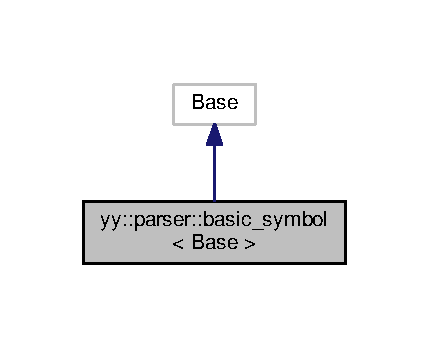
\includegraphics[width=206pt]{structyy_1_1parser_1_1basic__symbol__inherit__graph}
\end{center}
\end{figure}


Collaboration diagram for yy\+:\+:parser\+:\+:basic\+\_\+symbol$<$ Base $>$\+:\nopagebreak
\begin{figure}[H]
\begin{center}
\leavevmode
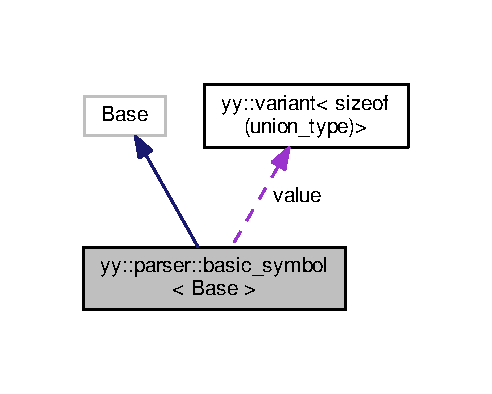
\includegraphics[width=236pt]{structyy_1_1parser_1_1basic__symbol__coll__graph}
\end{center}
\end{figure}
\subsection*{Public Types}
\begin{DoxyCompactItemize}
\item 
\hypertarget{structyy_1_1parser_1_1basic__symbol_aa67d0c9c65599dcf9d193b33743dae20}{}typedef Base \hyperlink{structyy_1_1parser_1_1basic__symbol_aa67d0c9c65599dcf9d193b33743dae20}{super\+\_\+type}\label{structyy_1_1parser_1_1basic__symbol_aa67d0c9c65599dcf9d193b33743dae20}

\begin{DoxyCompactList}\small\item\em Alias to Base. \end{DoxyCompactList}\end{DoxyCompactItemize}
\subsection*{Public Member Functions}
\begin{DoxyCompactItemize}
\item 
\hypertarget{structyy_1_1parser_1_1basic__symbol_a4c089d17ee545d109ca5660fbaa05b95}{}\hyperlink{structyy_1_1parser_1_1basic__symbol_a4c089d17ee545d109ca5660fbaa05b95}{basic\+\_\+symbol} ()\label{structyy_1_1parser_1_1basic__symbol_a4c089d17ee545d109ca5660fbaa05b95}

\begin{DoxyCompactList}\small\item\em Default constructor. \end{DoxyCompactList}\item 
\hypertarget{structyy_1_1parser_1_1basic__symbol_a840c58a9a75349d49586d6d0701dc0d9}{}\hyperlink{structyy_1_1parser_1_1basic__symbol_a840c58a9a75349d49586d6d0701dc0d9}{basic\+\_\+symbol} (const \hyperlink{structyy_1_1parser_1_1basic__symbol}{basic\+\_\+symbol} \&other)\label{structyy_1_1parser_1_1basic__symbol_a840c58a9a75349d49586d6d0701dc0d9}

\begin{DoxyCompactList}\small\item\em Copy constructor. \end{DoxyCompactList}\item 
\hypertarget{structyy_1_1parser_1_1basic__symbol_a20a558cd967a14b2645423110ed4f773}{}\hyperlink{structyy_1_1parser_1_1basic__symbol_a20a558cd967a14b2645423110ed4f773}{basic\+\_\+symbol} (typename Base\+::kind\+\_\+type t)\label{structyy_1_1parser_1_1basic__symbol_a20a558cd967a14b2645423110ed4f773}

\begin{DoxyCompactList}\small\item\em Constructor for valueless symbols, and symbols from each type. \end{DoxyCompactList}\item 
\hypertarget{structyy_1_1parser_1_1basic__symbol_a8a952ff44a513f5237fd81d038c0e0c2}{}{\bfseries basic\+\_\+symbol} (typename Base\+::kind\+\_\+type t, const \hyperlink{classNode}{Node} $\ast$v)\label{structyy_1_1parser_1_1basic__symbol_a8a952ff44a513f5237fd81d038c0e0c2}

\item 
\hypertarget{structyy_1_1parser_1_1basic__symbol_ade2aabbeb295bdadd1862239e8a7cda1}{}{\bfseries basic\+\_\+symbol} (typename Base\+::kind\+\_\+type t, const string v)\label{structyy_1_1parser_1_1basic__symbol_ade2aabbeb295bdadd1862239e8a7cda1}

\item 
\hypertarget{structyy_1_1parser_1_1basic__symbol_a56d8d7f7e389fa9e8eccaf36d61bf828}{}\hyperlink{structyy_1_1parser_1_1basic__symbol_a56d8d7f7e389fa9e8eccaf36d61bf828}{basic\+\_\+symbol} (typename Base\+::kind\+\_\+type t, const \hyperlink{classyy_1_1parser_a0ce15da9cf616a7197b81e6055428165}{semantic\+\_\+type} \&v)\label{structyy_1_1parser_1_1basic__symbol_a56d8d7f7e389fa9e8eccaf36d61bf828}

\begin{DoxyCompactList}\small\item\em Constructor for symbols with semantic value. \end{DoxyCompactList}\item 
\hypertarget{structyy_1_1parser_1_1basic__symbol_acd8919976d679380b4702a973134b4e3}{}void \hyperlink{structyy_1_1parser_1_1basic__symbol_acd8919976d679380b4702a973134b4e3}{move} (\hyperlink{structyy_1_1parser_1_1basic__symbol}{basic\+\_\+symbol} \&s)\label{structyy_1_1parser_1_1basic__symbol_acd8919976d679380b4702a973134b4e3}

\begin{DoxyCompactList}\small\item\em Destructive move, {\itshape s} is emptied into this. \end{DoxyCompactList}\end{DoxyCompactItemize}
\subsection*{Public Attributes}
\begin{DoxyCompactItemize}
\item 
\hypertarget{structyy_1_1parser_1_1basic__symbol_a07710fa55ed90f64504e2fe9b09802ca}{}\hyperlink{classyy_1_1parser_a0ce15da9cf616a7197b81e6055428165}{semantic\+\_\+type} \hyperlink{structyy_1_1parser_1_1basic__symbol_a07710fa55ed90f64504e2fe9b09802ca}{value}\label{structyy_1_1parser_1_1basic__symbol_a07710fa55ed90f64504e2fe9b09802ca}

\begin{DoxyCompactList}\small\item\em The semantic value. \end{DoxyCompactList}\end{DoxyCompactItemize}


\subsection{Detailed Description}
\subsubsection*{template$<$typename Base$>$struct yy\+::parser\+::basic\+\_\+symbol$<$ Base $>$}

A complete symbol. 

Expects its Base type to provide access to the symbol type via type\+\_\+get().

Provide access to semantic value. 

The documentation for this struct was generated from the following file\+:\begin{DoxyCompactItemize}
\item 
inc/\hyperlink{parser_8h}{parser.\+h}\end{DoxyCompactItemize}

\hypertarget{classBinop}{}\section{Binop Class Reference}
\label{classBinop}\index{Binop@{Binop}}


Handles binary operations.  




{\ttfamily \#include $<$Binop.\+h$>$}



Inheritance diagram for Binop\+:\nopagebreak
\begin{figure}[H]
\begin{center}
\leavevmode
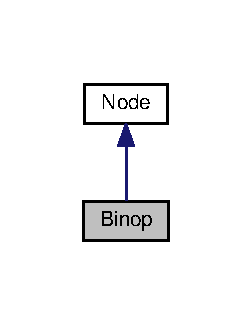
\includegraphics[width=121pt]{classBinop__inherit__graph}
\end{center}
\end{figure}


Collaboration diagram for Binop\+:\nopagebreak
\begin{figure}[H]
\begin{center}
\leavevmode
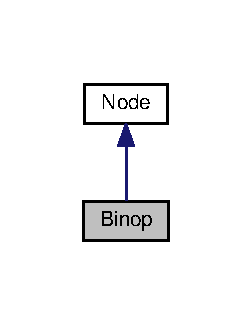
\includegraphics[width=121pt]{classBinop__coll__graph}
\end{center}
\end{figure}
\subsection*{Public Types}
\begin{DoxyCompactItemize}
\item 
\hypertarget{classBinop_a833e85c431d85ca69758bfebec9193dc}{}enum \hyperlink{classBinop_a833e85c431d85ca69758bfebec9193dc}{Type} \{ \\*
{\bfseries Undefined}, 
{\bfseries Equal}, 
{\bfseries Addition}, 
{\bfseries Subtraction}, 
\\*
{\bfseries Division}, 
{\bfseries Multiplication}, 
{\bfseries Power}, 
{\bfseries Modulo}
 \}\label{classBinop_a833e85c431d85ca69758bfebec9193dc}

\begin{DoxyCompactList}\small\item\em Defines types of Binops. \end{DoxyCompactList}\end{DoxyCompactItemize}
\subsection*{Public Member Functions}
\begin{DoxyCompactItemize}
\item 
\hypertarget{classBinop_a18bd9729a042a045df7fe11ffe068707}{}\hyperlink{classBinop_a18bd9729a042a045df7fe11ffe068707}{Binop} ()\label{classBinop_a18bd9729a042a045df7fe11ffe068707}

\begin{DoxyCompactList}\small\item\em Default constructor. \end{DoxyCompactList}\item 
\hyperlink{classBinop_a3d538d66e8aa1ac46feb5e984fbfb8c9}{Binop} (\hyperlink{classBinop_a833e85c431d85ca69758bfebec9193dc}{Type} \hyperlink{classBinop_a6ba1f508e1122caea1ef9350fee74396}{type})
\begin{DoxyCompactList}\small\item\em Constructor with type. \end{DoxyCompactList}\item 
bool \hyperlink{classBinop_ac3cff65931eaf4d542fc50c1dc696f55}{execute} (\hyperlink{classEnvironment}{Environment} \&env)
\begin{DoxyCompactList}\small\item\em Executes the \hyperlink{classNode}{Node}. \end{DoxyCompactList}\item 
int \hyperlink{classBinop_a5f011a9a0259af43447271dfc8668a2a}{eval\+Int} (\hyperlink{classEnvironment}{Environment} \&env)
\begin{DoxyCompactList}\small\item\em Evaluate integer of the \hyperlink{classBinop}{Binop}. \end{DoxyCompactList}\item 
std\+::string \hyperlink{classBinop_a9b31b3aa7963440e499143f8fb837bf4}{eval\+Str} (\hyperlink{classEnvironment}{Environment} \&env)
\begin{DoxyCompactList}\small\item\em Evaluate string of the \hyperlink{classBinop}{Binop}. \end{DoxyCompactList}\item 
std\+::string \hyperlink{classBinop_a25a4913ef0d2ec9787df24c391734094}{get\+Type} ()
\begin{DoxyCompactList}\small\item\em Converts type of node to string. \end{DoxyCompactList}\end{DoxyCompactItemize}
\subsection*{Protected Attributes}
\begin{DoxyCompactItemize}
\item 
\hypertarget{classBinop_a6ba1f508e1122caea1ef9350fee74396}{}\hyperlink{classBinop_a833e85c431d85ca69758bfebec9193dc}{Type} \hyperlink{classBinop_a6ba1f508e1122caea1ef9350fee74396}{type}\label{classBinop_a6ba1f508e1122caea1ef9350fee74396}

\begin{DoxyCompactList}\small\item\em \hyperlink{classBinop}{Binop} type. \end{DoxyCompactList}\end{DoxyCompactItemize}


\subsection{Detailed Description}
Handles binary operations. 

\begin{DoxyAuthor}{Author}
Jim Ahlstrand 
\end{DoxyAuthor}
\begin{DoxyRefDesc}{Todo}
\item[\hyperlink{todo__todo000001}{Todo}]add test for number of children, binop can have max 2 \end{DoxyRefDesc}


\subsection{Constructor \& Destructor Documentation}
\hypertarget{classBinop_a3d538d66e8aa1ac46feb5e984fbfb8c9}{}\index{Binop@{Binop}!Binop@{Binop}}
\index{Binop@{Binop}!Binop@{Binop}}
\subsubsection[{Binop}]{\setlength{\rightskip}{0pt plus 5cm}Binop\+::\+Binop (
\begin{DoxyParamCaption}
\item[{{\bf Type}}]{type}
\end{DoxyParamCaption}
)}\label{classBinop_a3d538d66e8aa1ac46feb5e984fbfb8c9}


Constructor with type. 


\begin{DoxyParams}{Parameters}
{\em type} & \hyperlink{classBinop}{Binop} type of enum Type \\
\hline
\end{DoxyParams}


\subsection{Member Function Documentation}
\hypertarget{classBinop_a5f011a9a0259af43447271dfc8668a2a}{}\index{Binop@{Binop}!eval\+Int@{eval\+Int}}
\index{eval\+Int@{eval\+Int}!Binop@{Binop}}
\subsubsection[{eval\+Int}]{\setlength{\rightskip}{0pt plus 5cm}int Binop\+::eval\+Int (
\begin{DoxyParamCaption}
\item[{{\bf Environment} \&}]{env}
\end{DoxyParamCaption}
)\hspace{0.3cm}{\ttfamily [virtual]}}\label{classBinop_a5f011a9a0259af43447271dfc8668a2a}


Evaluate integer of the \hyperlink{classBinop}{Binop}. 


\begin{DoxyParams}{Parameters}
{\em env} & current \hyperlink{classEnvironment}{Environment} \\
\hline
\end{DoxyParams}
\begin{DoxyReturn}{Returns}
integer value of the node 
\end{DoxyReturn}


Reimplemented from \hyperlink{classNode_ab5a9a064d1d0ef20c984b1d76e56d843}{Node}.

\hypertarget{classBinop_a9b31b3aa7963440e499143f8fb837bf4}{}\index{Binop@{Binop}!eval\+Str@{eval\+Str}}
\index{eval\+Str@{eval\+Str}!Binop@{Binop}}
\subsubsection[{eval\+Str}]{\setlength{\rightskip}{0pt plus 5cm}std\+::string Binop\+::eval\+Str (
\begin{DoxyParamCaption}
\item[{{\bf Environment} \&}]{env}
\end{DoxyParamCaption}
)\hspace{0.3cm}{\ttfamily [virtual]}}\label{classBinop_a9b31b3aa7963440e499143f8fb837bf4}


Evaluate string of the \hyperlink{classBinop}{Binop}. 


\begin{DoxyParams}{Parameters}
{\em env} & current \hyperlink{classEnvironment}{Environment} \\
\hline
\end{DoxyParams}
\begin{DoxyReturn}{Returns}
string value of the node
\end{DoxyReturn}
\begin{DoxyRemark}{Remarks}
this is ugly but works 
\end{DoxyRemark}


Reimplemented from \hyperlink{classNode_a8ee89abe1c903f5a0bae8ed3c798b47a}{Node}.

\hypertarget{classBinop_ac3cff65931eaf4d542fc50c1dc696f55}{}\index{Binop@{Binop}!execute@{execute}}
\index{execute@{execute}!Binop@{Binop}}
\subsubsection[{execute}]{\setlength{\rightskip}{0pt plus 5cm}bool Binop\+::execute (
\begin{DoxyParamCaption}
\item[{{\bf Environment} \&}]{env}
\end{DoxyParamCaption}
)\hspace{0.3cm}{\ttfamily [virtual]}}\label{classBinop_ac3cff65931eaf4d542fc50c1dc696f55}


Executes the \hyperlink{classNode}{Node}. 


\begin{DoxyParams}{Parameters}
{\em env} & current \hyperlink{classEnvironment}{Environment} \\
\hline
\end{DoxyParams}
\begin{DoxyReturn}{Returns}
bool true if node did execute
\end{DoxyReturn}
\begin{DoxyRemark}{Remarks}
This small limits expressions to integers 
\end{DoxyRemark}


Reimplemented from \hyperlink{classNode_ad2758f63dc60560b83e1d8a038df6e86}{Node}.

\hypertarget{classBinop_a25a4913ef0d2ec9787df24c391734094}{}\index{Binop@{Binop}!get\+Type@{get\+Type}}
\index{get\+Type@{get\+Type}!Binop@{Binop}}
\subsubsection[{get\+Type}]{\setlength{\rightskip}{0pt plus 5cm}std\+::string Binop\+::get\+Type (
\begin{DoxyParamCaption}
{}
\end{DoxyParamCaption}
)\hspace{0.3cm}{\ttfamily [virtual]}}\label{classBinop_a25a4913ef0d2ec9787df24c391734094}


Converts type of node to string. 

\begin{DoxyReturn}{Returns}
string type of the node 
\end{DoxyReturn}


Reimplemented from \hyperlink{classNode_abce0a9ddac6a5e2c0e546dbe6af02e3d}{Node}.



The documentation for this class was generated from the following files\+:\begin{DoxyCompactItemize}
\item 
inc/Binop.\+h\item 
src/Binop.\+cpp\end{DoxyCompactItemize}

\hypertarget{structyy_1_1parser_1_1by__type}{}\section{yy\+:\+:parser\+:\+:by\+\_\+type Struct Reference}
\label{structyy_1_1parser_1_1by__type}\index{yy\+::parser\+::by\+\_\+type@{yy\+::parser\+::by\+\_\+type}}


Type access provider for token (enum) based symbols.  




{\ttfamily \#include $<$parser.\+h$>$}

\subsection*{Public Types}
\begin{DoxyCompactItemize}
\item 
\hypertarget{structyy_1_1parser_1_1by__type_a101f5050061c63717e96210c68df732e}{}enum \{ {\bfseries empty} = 0
 \}\label{structyy_1_1parser_1_1by__type_a101f5050061c63717e96210c68df732e}

\item 
\hypertarget{structyy_1_1parser_1_1by__type_af8757490fd5397ad574e9fee1b80fa25}{}typedef \hyperlink{classyy_1_1parser_ac1ba3f834abfa251ea746c4ca8da5a85}{token\+\_\+type} \hyperlink{structyy_1_1parser_1_1by__type_af8757490fd5397ad574e9fee1b80fa25}{kind\+\_\+type}\label{structyy_1_1parser_1_1by__type_af8757490fd5397ad574e9fee1b80fa25}

\begin{DoxyCompactList}\small\item\em The symbol type as needed by the constructor. \end{DoxyCompactList}\end{DoxyCompactItemize}
\subsection*{Public Member Functions}
\begin{DoxyCompactItemize}
\item 
\hypertarget{structyy_1_1parser_1_1by__type_a16c7227367f85b611980ed547f545483}{}\hyperlink{structyy_1_1parser_1_1by__type_a16c7227367f85b611980ed547f545483}{by\+\_\+type} ()\label{structyy_1_1parser_1_1by__type_a16c7227367f85b611980ed547f545483}

\begin{DoxyCompactList}\small\item\em Default constructor. \end{DoxyCompactList}\item 
\hypertarget{structyy_1_1parser_1_1by__type_aa99c31c49c133c9ec3fe3f06ee30692c}{}\hyperlink{structyy_1_1parser_1_1by__type_aa99c31c49c133c9ec3fe3f06ee30692c}{by\+\_\+type} (const \hyperlink{structyy_1_1parser_1_1by__type}{by\+\_\+type} \&other)\label{structyy_1_1parser_1_1by__type_aa99c31c49c133c9ec3fe3f06ee30692c}

\begin{DoxyCompactList}\small\item\em Copy constructor. \end{DoxyCompactList}\item 
\hypertarget{structyy_1_1parser_1_1by__type_a7f43ae4d6b5ae70d2a7ef537c1ea42b2}{}\hyperlink{structyy_1_1parser_1_1by__type_a7f43ae4d6b5ae70d2a7ef537c1ea42b2}{by\+\_\+type} (\hyperlink{structyy_1_1parser_1_1by__type_af8757490fd5397ad574e9fee1b80fa25}{kind\+\_\+type} t)\label{structyy_1_1parser_1_1by__type_a7f43ae4d6b5ae70d2a7ef537c1ea42b2}

\begin{DoxyCompactList}\small\item\em Constructor from (external) token numbers. \end{DoxyCompactList}\item 
\hypertarget{structyy_1_1parser_1_1by__type_a68911dec3423e0748fd56f369d1b5d10}{}void \hyperlink{structyy_1_1parser_1_1by__type_a68911dec3423e0748fd56f369d1b5d10}{move} (\hyperlink{structyy_1_1parser_1_1by__type}{by\+\_\+type} \&that)\label{structyy_1_1parser_1_1by__type_a68911dec3423e0748fd56f369d1b5d10}

\begin{DoxyCompactList}\small\item\em Steal the symbol type from {\itshape that}. \end{DoxyCompactList}\item 
\hyperlink{classyy_1_1parser_a522f5c6c3481d9285b0b991ac12292eb}{symbol\+\_\+number\+\_\+type} \hyperlink{structyy_1_1parser_1_1by__type_a2324af0aef49d4a89ef346ebf5d66559}{type\+\_\+get} () const 
\item 
\hypertarget{structyy_1_1parser_1_1by__type_ab13b34d01faa03e8e5c24069aedaa225}{}\hyperlink{classyy_1_1parser_ac1ba3f834abfa251ea746c4ca8da5a85}{token\+\_\+type} \hyperlink{structyy_1_1parser_1_1by__type_ab13b34d01faa03e8e5c24069aedaa225}{token} () const \label{structyy_1_1parser_1_1by__type_ab13b34d01faa03e8e5c24069aedaa225}

\begin{DoxyCompactList}\small\item\em The token. \end{DoxyCompactList}\end{DoxyCompactItemize}
\subsection*{Public Attributes}
\begin{DoxyCompactItemize}
\item 
\hyperlink{classyy_1_1parser_a9e3963a210d7f2b655d87ca544223ead}{token\+\_\+number\+\_\+type} \hyperlink{structyy_1_1parser_1_1by__type_aecfb7b8174ce27df6dc0e6ef919bfb48}{type}
\end{DoxyCompactItemize}


\subsection{Detailed Description}
Type access provider for token (enum) based symbols. 

\subsection{Member Function Documentation}
\hypertarget{structyy_1_1parser_1_1by__type_a2324af0aef49d4a89ef346ebf5d66559}{}\index{yy\+::parser\+::by\+\_\+type@{yy\+::parser\+::by\+\_\+type}!type\+\_\+get@{type\+\_\+get}}
\index{type\+\_\+get@{type\+\_\+get}!yy\+::parser\+::by\+\_\+type@{yy\+::parser\+::by\+\_\+type}}
\subsubsection[{type\+\_\+get}]{\setlength{\rightskip}{0pt plus 5cm}int yy\+::parser\+::by\+\_\+type\+::type\+\_\+get (
\begin{DoxyParamCaption}
{}
\end{DoxyParamCaption}
) const\hspace{0.3cm}{\ttfamily [inline]}}\label{structyy_1_1parser_1_1by__type_a2324af0aef49d4a89ef346ebf5d66559}
The (internal) type number (corresponding to {\itshape type}). -\/1 when this symbol is empty. 

\subsection{Member Data Documentation}
\hypertarget{structyy_1_1parser_1_1by__type_aecfb7b8174ce27df6dc0e6ef919bfb48}{}\index{yy\+::parser\+::by\+\_\+type@{yy\+::parser\+::by\+\_\+type}!type@{type}}
\index{type@{type}!yy\+::parser\+::by\+\_\+type@{yy\+::parser\+::by\+\_\+type}}
\subsubsection[{type}]{\setlength{\rightskip}{0pt plus 5cm}{\bf token\+\_\+number\+\_\+type} yy\+::parser\+::by\+\_\+type\+::type}\label{structyy_1_1parser_1_1by__type_aecfb7b8174ce27df6dc0e6ef919bfb48}
The symbol type. -\/1 when this symbol is empty. 

The documentation for this struct was generated from the following file\+:\begin{DoxyCompactItemize}
\item 
inc/\hyperlink{parser_8h}{parser.\+h}\end{DoxyCompactItemize}

\hypertarget{classCondition}{}\section{Condition Class Reference}
\label{classCondition}\index{Condition@{Condition}}


Handles contitional operations.  




{\ttfamily \#include $<$Condition.\+h$>$}



Inheritance diagram for Condition\+:
\nopagebreak
\begin{figure}[H]
\begin{center}
\leavevmode
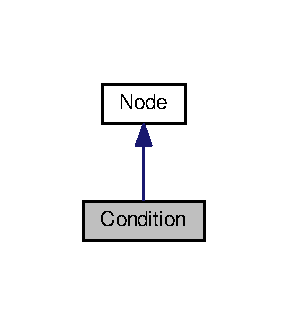
\includegraphics[width=138pt]{classCondition__inherit__graph}
\end{center}
\end{figure}


Collaboration diagram for Condition\+:
\nopagebreak
\begin{figure}[H]
\begin{center}
\leavevmode
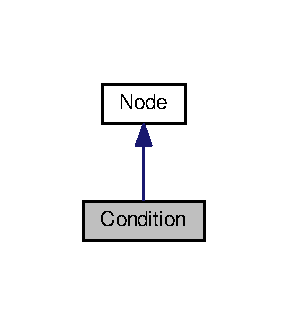
\includegraphics[width=138pt]{classCondition__coll__graph}
\end{center}
\end{figure}
\subsection*{Public Types}
\begin{DoxyCompactItemize}
\item 
\hypertarget{classCondition_a3eed4b7ef94da5dda4a3353cffa8266e}{}enum \hyperlink{classCondition_a3eed4b7ef94da5dda4a3353cffa8266e}{Type} \{ {\bfseries Undefined}, 
{\bfseries If}, 
{\bfseries Else\+If}
 \}\label{classCondition_a3eed4b7ef94da5dda4a3353cffa8266e}

\begin{DoxyCompactList}\small\item\em Defines types of Conditions. \end{DoxyCompactList}\end{DoxyCompactItemize}
\subsection*{Public Member Functions}
\begin{DoxyCompactItemize}
\item 
\hypertarget{classCondition_af11513db4fcbde93961fa0b65e7ab764}{}\hyperlink{classCondition_af11513db4fcbde93961fa0b65e7ab764}{Condition} ()\label{classCondition_af11513db4fcbde93961fa0b65e7ab764}

\begin{DoxyCompactList}\small\item\em Default constructor. \end{DoxyCompactList}\item 
\hyperlink{classCondition_adffecd1d1fac2e3e75e190c63b409dd1}{Condition} (\hyperlink{classCondition_a3eed4b7ef94da5dda4a3353cffa8266e}{Type} \hyperlink{classCondition_aeebc812b5f02a5e017c26d4573e85530}{type})
\begin{DoxyCompactList}\small\item\em Constructor with type. \end{DoxyCompactList}\item 
bool \hyperlink{classCondition_a4660fd89788efc03c57c35f66e14ae5b}{execute} (\hyperlink{classEnvironment}{Environment} \&env)
\begin{DoxyCompactList}\small\item\em Executes the \hyperlink{classCondition}{Condition}. \end{DoxyCompactList}\item 
std\+::string \hyperlink{classCondition_addf79a820326e04e58937c9875afe181}{get\+Type} ()
\begin{DoxyCompactList}\small\item\em Converts type of node to string. \end{DoxyCompactList}\end{DoxyCompactItemize}
\subsection*{Protected Attributes}
\begin{DoxyCompactItemize}
\item 
\hypertarget{classCondition_aeebc812b5f02a5e017c26d4573e85530}{}\hyperlink{classCondition_a3eed4b7ef94da5dda4a3353cffa8266e}{Type} \hyperlink{classCondition_aeebc812b5f02a5e017c26d4573e85530}{type}\label{classCondition_aeebc812b5f02a5e017c26d4573e85530}

\begin{DoxyCompactList}\small\item\em \hyperlink{classCondition}{Condition} type. \end{DoxyCompactList}\end{DoxyCompactItemize}


\subsection{Detailed Description}
Handles contitional operations. 

\begin{DoxyAuthor}{Author}
Jim Ahlstrand 
\end{DoxyAuthor}


\subsection{Constructor \& Destructor Documentation}
\hypertarget{classCondition_adffecd1d1fac2e3e75e190c63b409dd1}{}\index{Condition@{Condition}!Condition@{Condition}}
\index{Condition@{Condition}!Condition@{Condition}}
\subsubsection[{Condition}]{\setlength{\rightskip}{0pt plus 5cm}Condition\+::\+Condition (
\begin{DoxyParamCaption}
\item[{{\bf Type}}]{type}
\end{DoxyParamCaption}
)}\label{classCondition_adffecd1d1fac2e3e75e190c63b409dd1}


Constructor with type. 


\begin{DoxyParams}{Parameters}
{\em type} & \hyperlink{classCondition}{Condition} type of enum Type \\
\hline
\end{DoxyParams}


\subsection{Member Function Documentation}
\hypertarget{classCondition_a4660fd89788efc03c57c35f66e14ae5b}{}\index{Condition@{Condition}!execute@{execute}}
\index{execute@{execute}!Condition@{Condition}}
\subsubsection[{execute}]{\setlength{\rightskip}{0pt plus 5cm}bool Condition\+::execute (
\begin{DoxyParamCaption}
\item[{{\bf Environment} \&}]{env}
\end{DoxyParamCaption}
)\hspace{0.3cm}{\ttfamily [virtual]}}\label{classCondition_a4660fd89788efc03c57c35f66e14ae5b}


Executes the \hyperlink{classCondition}{Condition}. 


\begin{DoxyParams}{Parameters}
{\em env} & current \hyperlink{classEnvironment}{Environment} \\
\hline
\end{DoxyParams}
\begin{DoxyReturn}{Returns}
integer value of the node 
\end{DoxyReturn}


Reimplemented from \hyperlink{classNode_ad2758f63dc60560b83e1d8a038df6e86}{Node}.

\hypertarget{classCondition_addf79a820326e04e58937c9875afe181}{}\index{Condition@{Condition}!get\+Type@{get\+Type}}
\index{get\+Type@{get\+Type}!Condition@{Condition}}
\subsubsection[{get\+Type}]{\setlength{\rightskip}{0pt plus 5cm}std\+::string Condition\+::get\+Type (
\begin{DoxyParamCaption}
{}
\end{DoxyParamCaption}
)\hspace{0.3cm}{\ttfamily [virtual]}}\label{classCondition_addf79a820326e04e58937c9875afe181}


Converts type of node to string. 

\begin{DoxyReturn}{Returns}
string type of the node 
\end{DoxyReturn}


Reimplemented from \hyperlink{classNode_abce0a9ddac6a5e2c0e546dbe6af02e3d}{Node}.



The documentation for this class was generated from the following files\+:\begin{DoxyCompactItemize}
\item 
inc/Condition.\+h\item 
src/Condition.\+cpp\end{DoxyCompactItemize}

\hypertarget{classEnvironment}{}\section{Environment Class Reference}
\label{classEnvironment}\index{Environment@{Environment}}


Handles current memory scope.  




{\ttfamily \#include $<$Environment.\+h$>$}

\subsection*{Public Member Functions}
\begin{DoxyCompactItemize}
\item 
\hypertarget{classEnvironment_a8b427c4448d8b7536666837521b9e83d}{}\hyperlink{classEnvironment_a8b427c4448d8b7536666837521b9e83d}{Environment} ()\label{classEnvironment_a8b427c4448d8b7536666837521b9e83d}

\begin{DoxyCompactList}\small\item\em Default constructor. \end{DoxyCompactList}\item 
\hyperlink{classEnvironment_a030253266b5d549059c14984dfbb31da}{Environment} (\hyperlink{classEnvironment}{Environment} $\ast$parent)
\begin{DoxyCompactList}\small\item\em Constructor with parent scope. \end{DoxyCompactList}\item 
\hypertarget{classEnvironment_a8e294735187880dd3d59be10c425b29d}{}virtual \hyperlink{classEnvironment_a8e294735187880dd3d59be10c425b29d}{$\sim$\+Environment} ()\label{classEnvironment_a8e294735187880dd3d59be10c425b29d}

\begin{DoxyCompactList}\small\item\em Default destructor. \end{DoxyCompactList}\item 
int \hyperlink{classEnvironment_af7d70b4545df76070cb5d7a4699e0d04}{write} (std\+::string name, \hyperlink{classMemory}{Memory} $\ast$memory, bool local=false)
\begin{DoxyCompactList}\small\item\em Writes to memory. \end{DoxyCompactList}\item 
int \hyperlink{classEnvironment_a5ef0731380006123a7b339a9eb6c3f8e}{write} (std\+::string name, \hyperlink{classNode}{Node} $\ast$node, bool local=false)
\begin{DoxyCompactList}\small\item\em Writes to memory. \end{DoxyCompactList}\item 
\hyperlink{classMemory}{Memory} $\ast$ \hyperlink{classEnvironment_a44bfdd6aa66ff6503c57e5e89ee2dd9c}{read} (std\+::string name)
\begin{DoxyCompactList}\small\item\em reads from memory \end{DoxyCompactList}\end{DoxyCompactItemize}


\subsection{Detailed Description}
Handles current memory scope. 

\begin{DoxyAuthor}{Author}
Jim Ahlstrand 
\end{DoxyAuthor}
\begin{DoxyRemark}{Remarks}
no support for invisible variables 
\end{DoxyRemark}


\subsection{Constructor \& Destructor Documentation}
\hypertarget{classEnvironment_a030253266b5d549059c14984dfbb31da}{}\index{Environment@{Environment}!Environment@{Environment}}
\index{Environment@{Environment}!Environment@{Environment}}
\subsubsection[{Environment}]{\setlength{\rightskip}{0pt plus 5cm}Environment\+::\+Environment (
\begin{DoxyParamCaption}
\item[{{\bf Environment} $\ast$}]{parent}
\end{DoxyParamCaption}
)}\label{classEnvironment_a030253266b5d549059c14984dfbb31da}


Constructor with parent scope. 


\begin{DoxyParams}{Parameters}
{\em parent} & \hyperlink{classEnvironment}{Environment} parent scope \\
\hline
\end{DoxyParams}


\subsection{Member Function Documentation}
\hypertarget{classEnvironment_a44bfdd6aa66ff6503c57e5e89ee2dd9c}{}\index{Environment@{Environment}!read@{read}}
\index{read@{read}!Environment@{Environment}}
\subsubsection[{read}]{\setlength{\rightskip}{0pt plus 5cm}{\bf Memory} $\ast$ Environment\+::read (
\begin{DoxyParamCaption}
\item[{std\+::string}]{name}
\end{DoxyParamCaption}
)}\label{classEnvironment_a44bfdd6aa66ff6503c57e5e89ee2dd9c}


reads from memory 


\begin{DoxyParams}{Parameters}
{\em string} & name identifier \\
\hline
\end{DoxyParams}
\begin{DoxyReturn}{Returns}
integer value of the variable 
\end{DoxyReturn}
\hypertarget{classEnvironment_af7d70b4545df76070cb5d7a4699e0d04}{}\index{Environment@{Environment}!write@{write}}
\index{write@{write}!Environment@{Environment}}
\subsubsection[{write}]{\setlength{\rightskip}{0pt plus 5cm}int Environment\+::write (
\begin{DoxyParamCaption}
\item[{std\+::string}]{name, }
\item[{{\bf Memory} $\ast$}]{memory, }
\item[{bool}]{local = {\ttfamily false}}
\end{DoxyParamCaption}
)}\label{classEnvironment_af7d70b4545df76070cb5d7a4699e0d04}


Writes to memory. 


\begin{DoxyParams}{Parameters}
{\em string} & name identifier \\
\hline
{\em Memory$\ast$} & mem pointer to memory \\
\hline
\end{DoxyParams}
\begin{DoxyReturn}{Returns}
int 0 if success 
\end{DoxyReturn}
\hypertarget{classEnvironment_a5ef0731380006123a7b339a9eb6c3f8e}{}\index{Environment@{Environment}!write@{write}}
\index{write@{write}!Environment@{Environment}}
\subsubsection[{write}]{\setlength{\rightskip}{0pt plus 5cm}int Environment\+::write (
\begin{DoxyParamCaption}
\item[{std\+::string}]{name, }
\item[{{\bf Node} $\ast$}]{node, }
\item[{bool}]{local = {\ttfamily false}}
\end{DoxyParamCaption}
)}\label{classEnvironment_a5ef0731380006123a7b339a9eb6c3f8e}


Writes to memory. 


\begin{DoxyParams}{Parameters}
{\em string} & name identifier \\
\hline
{\em Node$\ast$} & node pointer that needs evaluation \\
\hline
\end{DoxyParams}
\begin{DoxyReturn}{Returns}
int 0 if success 
\end{DoxyReturn}
\begin{DoxyRemark}{Remarks}
Really ugly this one is 
\end{DoxyRemark}


The documentation for this class was generated from the following files\+:\begin{DoxyCompactItemize}
\item 
inc/Environment.\+h\item 
src/Environment.\+cpp\end{DoxyCompactItemize}

\hypertarget{classError}{}\section{Error Class Reference}
\label{classError}\index{Error@{Error}}


Class for handling simple errors.  




{\ttfamily \#include $<$Error.\+h$>$}



Inheritance diagram for Error\+:
\nopagebreak
\begin{figure}[H]
\begin{center}
\leavevmode
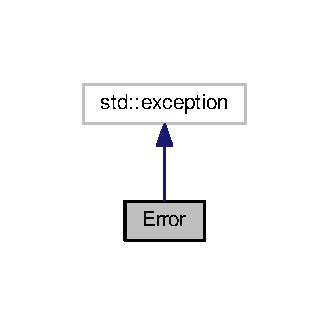
\includegraphics[width=158pt]{classError__inherit__graph}
\end{center}
\end{figure}


Collaboration diagram for Error\+:
\nopagebreak
\begin{figure}[H]
\begin{center}
\leavevmode
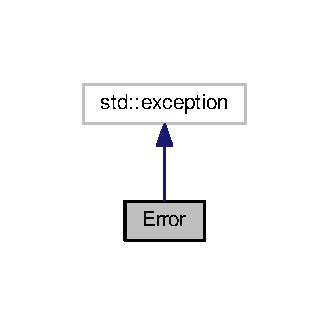
\includegraphics[width=158pt]{classError__coll__graph}
\end{center}
\end{figure}
\subsection*{Public Member Functions}
\begin{DoxyCompactItemize}
\item 
\hypertarget{classError_aa26df5de41c9f8b689b9f42fdbbc9abd}{}\hyperlink{classError_aa26df5de41c9f8b689b9f42fdbbc9abd}{Error} (std\+::string msg)\label{classError_aa26df5de41c9f8b689b9f42fdbbc9abd}

\begin{DoxyCompactList}\small\item\em Constructor with msg. \end{DoxyCompactList}\item 
const char $\ast$ \hyperlink{classError_a57dd37fd445e3182ed9da6ebfd2a28c0}{what} ()
\begin{DoxyCompactList}\small\item\em Overloads the what function. \end{DoxyCompactList}\end{DoxyCompactItemize}


\subsection{Detailed Description}
Class for handling simple errors. 

\begin{DoxyAuthor}{Author}
Jim Ahlstrand 
\end{DoxyAuthor}


\subsection{Member Function Documentation}
\hypertarget{classError_a57dd37fd445e3182ed9da6ebfd2a28c0}{}\index{Error@{Error}!what@{what}}
\index{what@{what}!Error@{Error}}
\subsubsection[{what}]{\setlength{\rightskip}{0pt plus 5cm}const char$\ast$ Error\+::what (
\begin{DoxyParamCaption}
{}
\end{DoxyParamCaption}
)\hspace{0.3cm}{\ttfamily [inline]}}\label{classError_a57dd37fd445e3182ed9da6ebfd2a28c0}


Overloads the what function. 

\begin{DoxyReturn}{Returns}
pointer to error message 
\end{DoxyReturn}


The documentation for this class was generated from the following file\+:\begin{DoxyCompactItemize}
\item 
inc/Error.\+h\end{DoxyCompactItemize}

\hypertarget{classLoop}{}\section{Loop Class Reference}
\label{classLoop}\index{Loop@{Loop}}


Handles loops.  




{\ttfamily \#include $<$Loop.\+h$>$}



Inheritance diagram for Loop\+:\nopagebreak
\begin{figure}[H]
\begin{center}
\leavevmode
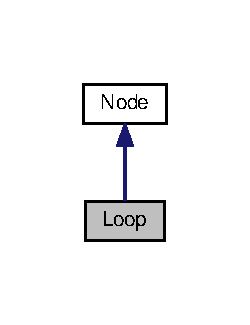
\includegraphics[width=120pt]{classLoop__inherit__graph}
\end{center}
\end{figure}


Collaboration diagram for Loop\+:\nopagebreak
\begin{figure}[H]
\begin{center}
\leavevmode
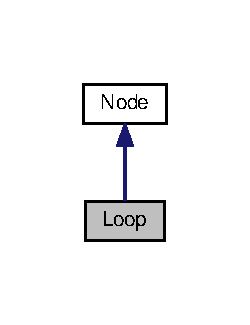
\includegraphics[width=120pt]{classLoop__coll__graph}
\end{center}
\end{figure}
\subsection*{Public Types}
\begin{DoxyCompactItemize}
\item 
\hypertarget{classLoop_af57e9c094063c514758dfe7bd986d6e7}{}enum \hyperlink{classLoop_af57e9c094063c514758dfe7bd986d6e7}{Type} \{ \\*
{\bfseries Undefined}, 
{\bfseries Repeat}, 
{\bfseries While}, 
{\bfseries For}, 
\\*
{\bfseries Do}
 \}\label{classLoop_af57e9c094063c514758dfe7bd986d6e7}

\begin{DoxyCompactList}\small\item\em Defines types of Loops. \end{DoxyCompactList}\end{DoxyCompactItemize}
\subsection*{Public Member Functions}
\begin{DoxyCompactItemize}
\item 
\hypertarget{classLoop_a675e74b960c5e703adf1ee0e6fd8f3bf}{}\hyperlink{classLoop_a675e74b960c5e703adf1ee0e6fd8f3bf}{Loop} ()\label{classLoop_a675e74b960c5e703adf1ee0e6fd8f3bf}

\begin{DoxyCompactList}\small\item\em Default constructor. \end{DoxyCompactList}\item 
\hyperlink{classLoop_a3e42ab398babe1ba79e9242d64147960}{Loop} (\hyperlink{classLoop_af57e9c094063c514758dfe7bd986d6e7}{Type} \hyperlink{classLoop_ae5e7c727c194b408bfc69b3f218c8b6f}{type})
\begin{DoxyCompactList}\small\item\em Constructor with type. \end{DoxyCompactList}\item 
bool \hyperlink{classLoop_a661edc5e6b0f90787e2a55922109f110}{execute} (\hyperlink{classEnvironment}{Environment} \&env)
\begin{DoxyCompactList}\small\item\em Executes the \hyperlink{classLoop}{Loop}. \end{DoxyCompactList}\item 
std\+::string \hyperlink{classLoop_a657b90074652fce7ab2028bdc3747b7b}{get\+Type} ()
\begin{DoxyCompactList}\small\item\em Converts type of node to string. \end{DoxyCompactList}\end{DoxyCompactItemize}
\subsection*{Protected Attributes}
\begin{DoxyCompactItemize}
\item 
\hypertarget{classLoop_ae5e7c727c194b408bfc69b3f218c8b6f}{}\hyperlink{classLoop_af57e9c094063c514758dfe7bd986d6e7}{Type} \hyperlink{classLoop_ae5e7c727c194b408bfc69b3f218c8b6f}{type}\label{classLoop_ae5e7c727c194b408bfc69b3f218c8b6f}

\begin{DoxyCompactList}\small\item\em \hyperlink{classLoop}{Loop} type. \end{DoxyCompactList}\end{DoxyCompactItemize}


\subsection{Detailed Description}
Handles loops. 

\begin{DoxyAuthor}{Author}
Jim Ahlstrand 
\end{DoxyAuthor}


\subsection{Constructor \& Destructor Documentation}
\hypertarget{classLoop_a3e42ab398babe1ba79e9242d64147960}{}\index{Loop@{Loop}!Loop@{Loop}}
\index{Loop@{Loop}!Loop@{Loop}}
\subsubsection[{Loop}]{\setlength{\rightskip}{0pt plus 5cm}Loop\+::\+Loop (
\begin{DoxyParamCaption}
\item[{{\bf Type}}]{type}
\end{DoxyParamCaption}
)}\label{classLoop_a3e42ab398babe1ba79e9242d64147960}


Constructor with type. 


\begin{DoxyParams}{Parameters}
{\em type} & \hyperlink{classLoop}{Loop} type of enum Type \\
\hline
\end{DoxyParams}


\subsection{Member Function Documentation}
\hypertarget{classLoop_a661edc5e6b0f90787e2a55922109f110}{}\index{Loop@{Loop}!execute@{execute}}
\index{execute@{execute}!Loop@{Loop}}
\subsubsection[{execute}]{\setlength{\rightskip}{0pt plus 5cm}bool Loop\+::execute (
\begin{DoxyParamCaption}
\item[{{\bf Environment} \&}]{env}
\end{DoxyParamCaption}
)\hspace{0.3cm}{\ttfamily [virtual]}}\label{classLoop_a661edc5e6b0f90787e2a55922109f110}


Executes the \hyperlink{classLoop}{Loop}. 


\begin{DoxyParams}{Parameters}
{\em env} & current \hyperlink{classEnvironment}{Environment} \\
\hline
\end{DoxyParams}
\begin{DoxyReturn}{Returns}
integer value of the node 
\end{DoxyReturn}
\begin{DoxyRefDesc}{Todo}
\item[\hyperlink{todo__todo000005}{Todo}]implement for loop execution \end{DoxyRefDesc}


\begin{DoxyRefDesc}{Todo}
\item[\hyperlink{todo__todo000006}{Todo}]implement do loop execution \end{DoxyRefDesc}


Reimplemented from \hyperlink{classNode_ad2758f63dc60560b83e1d8a038df6e86}{Node}.

\hypertarget{classLoop_a657b90074652fce7ab2028bdc3747b7b}{}\index{Loop@{Loop}!get\+Type@{get\+Type}}
\index{get\+Type@{get\+Type}!Loop@{Loop}}
\subsubsection[{get\+Type}]{\setlength{\rightskip}{0pt plus 5cm}std\+::string Loop\+::get\+Type (
\begin{DoxyParamCaption}
{}
\end{DoxyParamCaption}
)\hspace{0.3cm}{\ttfamily [virtual]}}\label{classLoop_a657b90074652fce7ab2028bdc3747b7b}


Converts type of node to string. 

\begin{DoxyReturn}{Returns}
string type of the node 
\end{DoxyReturn}


Reimplemented from \hyperlink{classNode_abce0a9ddac6a5e2c0e546dbe6af02e3d}{Node}.



The documentation for this class was generated from the following files\+:\begin{DoxyCompactItemize}
\item 
inc/Loop.\+h\item 
src/Loop.\+cpp\end{DoxyCompactItemize}

\hypertarget{classMemory}{}\section{Memory Class Reference}
\label{classMemory}\index{Memory@{Memory}}


Handles memory operations.  




{\ttfamily \#include $<$Memory.\+h$>$}



Inheritance diagram for Memory\+:
\nopagebreak
\begin{figure}[H]
\begin{center}
\leavevmode
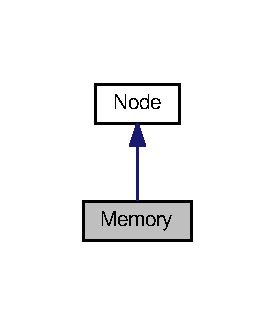
\includegraphics[width=132pt]{classMemory__inherit__graph}
\end{center}
\end{figure}


Collaboration diagram for Memory\+:
\nopagebreak
\begin{figure}[H]
\begin{center}
\leavevmode
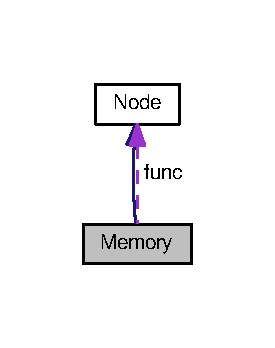
\includegraphics[width=132pt]{classMemory__coll__graph}
\end{center}
\end{figure}
\subsection*{Public Types}
\begin{DoxyCompactItemize}
\item 
\hypertarget{classMemory_a9193c3e610b1728964440284db90c812}{}enum \hyperlink{classMemory_a9193c3e610b1728964440284db90c812}{Type} \{ \\*
{\bfseries Nil}, 
{\bfseries Number}, 
{\bfseries String}, 
{\bfseries Function}, 
\\*
{\bfseries Field\+List}
 \}\label{classMemory_a9193c3e610b1728964440284db90c812}

\begin{DoxyCompactList}\small\item\em Defines types of \hyperlink{classMemory}{Memory}. \end{DoxyCompactList}\end{DoxyCompactItemize}
\subsection*{Public Member Functions}
\begin{DoxyCompactItemize}
\item 
\hyperlink{classMemory_a585d7bb6fc6f2237bcebf94a86b7dd99}{Memory} ()
\begin{DoxyCompactList}\small\item\em Default constructor. \end{DoxyCompactList}\item 
\hyperlink{classMemory_a94bd3f09f65c210e6f4259724d2b8efa}{Memory} (int \hyperlink{classNode_a51de8a12e67206f893b0bd6c2afeb11c}{value})
\begin{DoxyCompactList}\small\item\em Constructor with integer type. \end{DoxyCompactList}\item 
\hyperlink{classMemory_a0174eface9607ffd7a5c40761ba09b1f}{Memory} (std\+::string \hyperlink{classNode_a51de8a12e67206f893b0bd6c2afeb11c}{value})
\begin{DoxyCompactList}\small\item\em Constructor with string type. \end{DoxyCompactList}\item 
\hyperlink{classMemory_a97531dd41f355d34c6479d9ebfd4b652}{Memory} (\hyperlink{classNode}{Node} $\ast$\hyperlink{classMemory_ae8c01f737989b477cf085612795ed13b}{func})
\begin{DoxyCompactList}\small\item\em Constructor with function type. \end{DoxyCompactList}\item 
\hypertarget{classMemory_a0ffa9759ebbf103f11132a505b93bdc0}{}virtual \hyperlink{classMemory_a0ffa9759ebbf103f11132a505b93bdc0}{$\sim$\+Memory} ()\label{classMemory_a0ffa9759ebbf103f11132a505b93bdc0}

\begin{DoxyCompactList}\small\item\em Default destructor. \end{DoxyCompactList}\item 
bool \hyperlink{classMemory_ae00c898b45732c0bf74140d604363319}{execute} (\hyperlink{classEnvironment}{Environment} \&env)
\begin{DoxyCompactList}\small\item\em Executes the \hyperlink{classNode}{Node}. \end{DoxyCompactList}\item 
int \hyperlink{classMemory_a0bf9b7657489146568ae62137c684522}{eval\+Int} (\hyperlink{classEnvironment}{Environment} \&env)
\begin{DoxyCompactList}\small\item\em Evaluate integer of the \hyperlink{classMemory}{Memory}. \end{DoxyCompactList}\item 
std\+::string \hyperlink{classMemory_a298bdf094ac4807ad563f76f5bf159d0}{eval\+Str} (\hyperlink{classEnvironment}{Environment} \&env)
\begin{DoxyCompactList}\small\item\em Evaluate string of the \hyperlink{classMemory}{Memory}. \end{DoxyCompactList}\item 
std\+::string \hyperlink{classMemory_a222e2dc37b587f8c243aabc1eebcf7a1}{get\+Type} ()
\begin{DoxyCompactList}\small\item\em Converts type of node to string. \end{DoxyCompactList}\item 
\hyperlink{classNode}{Node} $\ast$ \hyperlink{classMemory_a45c7902075f19101c539240893075311}{get\+Func} ()
\begin{DoxyCompactList}\small\item\em Gets the function pointer. \end{DoxyCompactList}\item 
int \hyperlink{classMemory_a4e22f8404e11645dcaa68b2ffc4c4455}{get\+Int} ()
\begin{DoxyCompactList}\small\item\em Gets the integer value. \end{DoxyCompactList}\item 
std\+::string \hyperlink{classMemory_aecf23bb53fc58d668edae8e4e791ea99}{get\+Str} ()
\begin{DoxyCompactList}\small\item\em Gets the string value. \end{DoxyCompactList}\item 
unsigned int \hyperlink{classMemory_a55d46c565490996d8680cdb78cca6a76}{length} ()
\begin{DoxyCompactList}\small\item\em Get length of \hyperlink{classMemory}{Memory}. \end{DoxyCompactList}\end{DoxyCompactItemize}
\subsection*{Protected Attributes}
\begin{DoxyCompactItemize}
\item 
\hypertarget{classMemory_a918d8160ac6fefa393ab29a11da83e6e}{}\hyperlink{classMemory_a9193c3e610b1728964440284db90c812}{Type} \hyperlink{classMemory_a918d8160ac6fefa393ab29a11da83e6e}{type}\label{classMemory_a918d8160ac6fefa393ab29a11da83e6e}

\begin{DoxyCompactList}\small\item\em \hyperlink{classMemory}{Memory} type. \end{DoxyCompactList}\item 
\hypertarget{classMemory_ac80bb688056b1ea413f35e6395e7c590}{}int \hyperlink{classMemory_ac80bb688056b1ea413f35e6395e7c590}{integer}\label{classMemory_ac80bb688056b1ea413f35e6395e7c590}

\begin{DoxyCompactList}\small\item\em Integer value. \end{DoxyCompactList}\item 
\hypertarget{classMemory_a96bb9384b8d7a57c75af4f1345279cc4}{}std\+::string \hyperlink{classMemory_a96bb9384b8d7a57c75af4f1345279cc4}{str}\label{classMemory_a96bb9384b8d7a57c75af4f1345279cc4}

\begin{DoxyCompactList}\small\item\em String value. \end{DoxyCompactList}\item 
\hypertarget{classMemory_ae8c01f737989b477cf085612795ed13b}{}\hyperlink{classNode}{Node} $\ast$ \hyperlink{classMemory_ae8c01f737989b477cf085612795ed13b}{func}\label{classMemory_ae8c01f737989b477cf085612795ed13b}

\begin{DoxyCompactList}\small\item\em Function pointer. \end{DoxyCompactList}\end{DoxyCompactItemize}


\subsection{Detailed Description}
Handles memory operations. 

\begin{DoxyAuthor}{Author}
Jim Ahlstrand 
\end{DoxyAuthor}
\begin{DoxyRefDesc}{Todo}
\item[\hyperlink{todo__todo000004}{Todo}]implement support for float variables and infinite large int \end{DoxyRefDesc}


\subsection{Constructor \& Destructor Documentation}
\hypertarget{classMemory_a585d7bb6fc6f2237bcebf94a86b7dd99}{}\index{Memory@{Memory}!Memory@{Memory}}
\index{Memory@{Memory}!Memory@{Memory}}
\subsubsection[{Memory}]{\setlength{\rightskip}{0pt plus 5cm}Memory\+::\+Memory (
\begin{DoxyParamCaption}
{}
\end{DoxyParamCaption}
)}\label{classMemory_a585d7bb6fc6f2237bcebf94a86b7dd99}


Default constructor. 

\begin{DoxyRemark}{Remarks}
is assumed to be a field list 
\end{DoxyRemark}
\hypertarget{classMemory_a94bd3f09f65c210e6f4259724d2b8efa}{}\index{Memory@{Memory}!Memory@{Memory}}
\index{Memory@{Memory}!Memory@{Memory}}
\subsubsection[{Memory}]{\setlength{\rightskip}{0pt plus 5cm}Memory\+::\+Memory (
\begin{DoxyParamCaption}
\item[{int}]{value}
\end{DoxyParamCaption}
)}\label{classMemory_a94bd3f09f65c210e6f4259724d2b8efa}


Constructor with integer type. 


\begin{DoxyParams}{Parameters}
{\em type} & \hyperlink{classMemory}{Memory} type of enum Type \\
\hline
{\em value} & integer value of the node \\
\hline
\end{DoxyParams}
\hypertarget{classMemory_a0174eface9607ffd7a5c40761ba09b1f}{}\index{Memory@{Memory}!Memory@{Memory}}
\index{Memory@{Memory}!Memory@{Memory}}
\subsubsection[{Memory}]{\setlength{\rightskip}{0pt plus 5cm}Memory\+::\+Memory (
\begin{DoxyParamCaption}
\item[{std\+::string}]{value}
\end{DoxyParamCaption}
)}\label{classMemory_a0174eface9607ffd7a5c40761ba09b1f}


Constructor with string type. 


\begin{DoxyParams}{Parameters}
{\em type} & \hyperlink{classMemory}{Memory} type of enum Type \\
\hline
{\em value} & string value of the node \\
\hline
\end{DoxyParams}
\hypertarget{classMemory_a97531dd41f355d34c6479d9ebfd4b652}{}\index{Memory@{Memory}!Memory@{Memory}}
\index{Memory@{Memory}!Memory@{Memory}}
\subsubsection[{Memory}]{\setlength{\rightskip}{0pt plus 5cm}Memory\+::\+Memory (
\begin{DoxyParamCaption}
\item[{{\bf Node} $\ast$}]{func}
\end{DoxyParamCaption}
)}\label{classMemory_a97531dd41f355d34c6479d9ebfd4b652}


Constructor with function type. 


\begin{DoxyParams}{Parameters}
{\em type} & \hyperlink{classMemory}{Memory} type of enum Type \\
\hline
{\em func} & Node$\ast$ value of the node \\
\hline
\end{DoxyParams}


\subsection{Member Function Documentation}
\hypertarget{classMemory_a0bf9b7657489146568ae62137c684522}{}\index{Memory@{Memory}!eval\+Int@{eval\+Int}}
\index{eval\+Int@{eval\+Int}!Memory@{Memory}}
\subsubsection[{eval\+Int}]{\setlength{\rightskip}{0pt plus 5cm}int Memory\+::eval\+Int (
\begin{DoxyParamCaption}
\item[{{\bf Environment} \&}]{env}
\end{DoxyParamCaption}
)\hspace{0.3cm}{\ttfamily [virtual]}}\label{classMemory_a0bf9b7657489146568ae62137c684522}


Evaluate integer of the \hyperlink{classMemory}{Memory}. 


\begin{DoxyParams}{Parameters}
{\em env} & current \hyperlink{classEnvironment}{Environment} \\
\hline
\end{DoxyParams}
\begin{DoxyReturn}{Returns}
integer value of the node 
\end{DoxyReturn}


Reimplemented from \hyperlink{classNode_ab5a9a064d1d0ef20c984b1d76e56d843}{Node}.

\hypertarget{classMemory_a298bdf094ac4807ad563f76f5bf159d0}{}\index{Memory@{Memory}!eval\+Str@{eval\+Str}}
\index{eval\+Str@{eval\+Str}!Memory@{Memory}}
\subsubsection[{eval\+Str}]{\setlength{\rightskip}{0pt plus 5cm}std\+::string Memory\+::eval\+Str (
\begin{DoxyParamCaption}
\item[{{\bf Environment} \&}]{env}
\end{DoxyParamCaption}
)\hspace{0.3cm}{\ttfamily [virtual]}}\label{classMemory_a298bdf094ac4807ad563f76f5bf159d0}


Evaluate string of the \hyperlink{classMemory}{Memory}. 


\begin{DoxyParams}{Parameters}
{\em env} & current \hyperlink{classEnvironment}{Environment} \\
\hline
\end{DoxyParams}
\begin{DoxyReturn}{Returns}
string value of the node 
\end{DoxyReturn}


Reimplemented from \hyperlink{classNode_a8ee89abe1c903f5a0bae8ed3c798b47a}{Node}.

\hypertarget{classMemory_ae00c898b45732c0bf74140d604363319}{}\index{Memory@{Memory}!execute@{execute}}
\index{execute@{execute}!Memory@{Memory}}
\subsubsection[{execute}]{\setlength{\rightskip}{0pt plus 5cm}bool Memory\+::execute (
\begin{DoxyParamCaption}
\item[{{\bf Environment} \&}]{env}
\end{DoxyParamCaption}
)\hspace{0.3cm}{\ttfamily [virtual]}}\label{classMemory_ae00c898b45732c0bf74140d604363319}


Executes the \hyperlink{classNode}{Node}. 


\begin{DoxyParams}{Parameters}
{\em env} & current \hyperlink{classEnvironment}{Environment} \\
\hline
\end{DoxyParams}
\begin{DoxyReturn}{Returns}
bool true if node did execute 
\end{DoxyReturn}


Reimplemented from \hyperlink{classNode_ad2758f63dc60560b83e1d8a038df6e86}{Node}.

\hypertarget{classMemory_a45c7902075f19101c539240893075311}{}\index{Memory@{Memory}!get\+Func@{get\+Func}}
\index{get\+Func@{get\+Func}!Memory@{Memory}}
\subsubsection[{get\+Func}]{\setlength{\rightskip}{0pt plus 5cm}{\bf Node}$\ast$ Memory\+::get\+Func (
\begin{DoxyParamCaption}
{}
\end{DoxyParamCaption}
)\hspace{0.3cm}{\ttfamily [inline]}}\label{classMemory_a45c7902075f19101c539240893075311}


Gets the function pointer. 

\begin{DoxyReturn}{Returns}
Node$\ast$ pointer to the function node 
\end{DoxyReturn}
\hypertarget{classMemory_a4e22f8404e11645dcaa68b2ffc4c4455}{}\index{Memory@{Memory}!get\+Int@{get\+Int}}
\index{get\+Int@{get\+Int}!Memory@{Memory}}
\subsubsection[{get\+Int}]{\setlength{\rightskip}{0pt plus 5cm}int Memory\+::get\+Int (
\begin{DoxyParamCaption}
{}
\end{DoxyParamCaption}
)\hspace{0.3cm}{\ttfamily [inline]}}\label{classMemory_a4e22f8404e11645dcaa68b2ffc4c4455}


Gets the integer value. 

\begin{DoxyReturn}{Returns}
integer 
\end{DoxyReturn}
\hypertarget{classMemory_aecf23bb53fc58d668edae8e4e791ea99}{}\index{Memory@{Memory}!get\+Str@{get\+Str}}
\index{get\+Str@{get\+Str}!Memory@{Memory}}
\subsubsection[{get\+Str}]{\setlength{\rightskip}{0pt plus 5cm}std\+::string Memory\+::get\+Str (
\begin{DoxyParamCaption}
{}
\end{DoxyParamCaption}
)\hspace{0.3cm}{\ttfamily [inline]}}\label{classMemory_aecf23bb53fc58d668edae8e4e791ea99}


Gets the string value. 

\begin{DoxyReturn}{Returns}
string 
\end{DoxyReturn}
\hypertarget{classMemory_a222e2dc37b587f8c243aabc1eebcf7a1}{}\index{Memory@{Memory}!get\+Type@{get\+Type}}
\index{get\+Type@{get\+Type}!Memory@{Memory}}
\subsubsection[{get\+Type}]{\setlength{\rightskip}{0pt plus 5cm}std\+::string Memory\+::get\+Type (
\begin{DoxyParamCaption}
{}
\end{DoxyParamCaption}
)\hspace{0.3cm}{\ttfamily [virtual]}}\label{classMemory_a222e2dc37b587f8c243aabc1eebcf7a1}


Converts type of node to string. 

\begin{DoxyReturn}{Returns}
string type of the node 
\end{DoxyReturn}


Reimplemented from \hyperlink{classNode_abce0a9ddac6a5e2c0e546dbe6af02e3d}{Node}.

\hypertarget{classMemory_a55d46c565490996d8680cdb78cca6a76}{}\index{Memory@{Memory}!length@{length}}
\index{length@{length}!Memory@{Memory}}
\subsubsection[{length}]{\setlength{\rightskip}{0pt plus 5cm}unsigned int Memory\+::length (
\begin{DoxyParamCaption}
{}
\end{DoxyParamCaption}
)}\label{classMemory_a55d46c565490996d8680cdb78cca6a76}


Get length of \hyperlink{classMemory}{Memory}. 

\begin{DoxyReturn}{Returns}
unsigned int length of \hyperlink{classMemory}{Memory} 
\end{DoxyReturn}
\begin{DoxyRemark}{Remarks}
length of list returns number of elements in list 

length of string returns number of characters in string 

length of integer \& function throws an exception 
\end{DoxyRemark}


The documentation for this class was generated from the following files\+:\begin{DoxyCompactItemize}
\item 
inc/Memory.\+h\item 
src/Memory.\+cpp\end{DoxyCompactItemize}

\hypertarget{classNode}{}\section{Node Class Reference}
\label{classNode}\index{Node@{Node}}


Builds a tree-\/node structure.  




{\ttfamily \#include $<$Node.\+h$>$}



Inheritance diagram for Node\+:\nopagebreak
\begin{figure}[H]
\begin{center}
\leavevmode
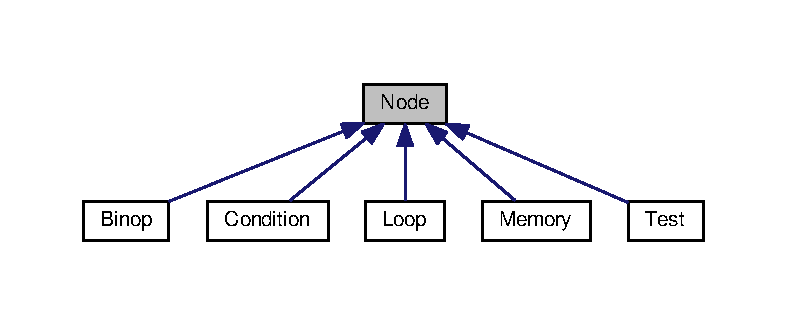
\includegraphics[width=350pt]{classNode__inherit__graph}
\end{center}
\end{figure}
\subsection*{Public Types}
\begin{DoxyCompactItemize}
\item 
enum \hyperlink{classNode_a8dad370be1595f49e0a7c2406a91e867}{Type} \{ \\*
{\bfseries Undefined}, 
{\bfseries Expression\+List}, 
\hyperlink{classNode_a8dad370be1595f49e0a7c2406a91e867a8fb6b35a2762acd63c8d42fc8575889e}{Variable\+List}, 
\hyperlink{classNode_a8dad370be1595f49e0a7c2406a91e867a496a823a62742a6ebb9f4fb757e02ce4}{Function\+Name}, 
\\*
{\bfseries Function\+Call}, 
{\bfseries Function\+Body}, 
{\bfseries Function}, 
{\bfseries Member\+Function}, 
\\*
\hyperlink{classNode_a8dad370be1595f49e0a7c2406a91e867a1a3ec9cbafad290cdd86122121b61391}{List\+Name}, 
\hyperlink{classNode_a8dad370be1595f49e0a7c2406a91e867a82f82cd405ee2ded93d8f9133e2f5f34}{Stat}, 
{\bfseries Field}, 
\hyperlink{classNode_a8dad370be1595f49e0a7c2406a91e867a12f1dc625982c23638509a4039543b59}{Field\+Element}, 
\\*
\hyperlink{classNode_a8dad370be1595f49e0a7c2406a91e867a9b98ce84dc5f406e0743acc13f03aaf6}{Double\+Dot}, 
\hyperlink{classNode_a8dad370be1595f49e0a7c2406a91e867ad05e3fa202cceccd870b5aac8467623c}{Hash}, 
{\bfseries Negate}, 
\hyperlink{classNode_a8dad370be1595f49e0a7c2406a91e867a183ed1e4cc2be1e5df44762c452281ef}{Name}, 
\\*
{\bfseries Tridot}, 
\hyperlink{classNode_a8dad370be1595f49e0a7c2406a91e867aab13754f7d035f904f4fc861bc6ad211}{Return}, 
\hyperlink{classNode_a8dad370be1595f49e0a7c2406a91e867a0636a6d172da086b233f0170ba995a81}{Do}
 \}
\begin{DoxyCompactList}\small\item\em Defines types of Nodes. \end{DoxyCompactList}\end{DoxyCompactItemize}
\subsection*{Public Member Functions}
\begin{DoxyCompactItemize}
\item 
\hypertarget{classNode_ad7a34779cad45d997bfd6d3d8043c75f}{}\hyperlink{classNode_ad7a34779cad45d997bfd6d3d8043c75f}{Node} ()\label{classNode_ad7a34779cad45d997bfd6d3d8043c75f}

\begin{DoxyCompactList}\small\item\em Default constructor. \end{DoxyCompactList}\item 
\hyperlink{classNode_a4122dca231612c6fd2eb17fd92a02892}{Node} (\hyperlink{classNode_a8dad370be1595f49e0a7c2406a91e867}{Type} \hyperlink{classNode_adcaf01927a597ad0e6025b173fe5e552}{type})
\begin{DoxyCompactList}\small\item\em Constructor with type. \end{DoxyCompactList}\item 
\hyperlink{classNode_a36ce067b8b3fde59af074a425fa3b97c}{Node} (\hyperlink{classNode_a8dad370be1595f49e0a7c2406a91e867}{Type} \hyperlink{classNode_adcaf01927a597ad0e6025b173fe5e552}{type}, std\+::string \hyperlink{classNode_a51de8a12e67206f893b0bd6c2afeb11c}{value})
\begin{DoxyCompactList}\small\item\em Constructor with type and value. \end{DoxyCompactList}\item 
\hypertarget{classNode_aa0840c3cb5c7159be6d992adecd2097c}{}virtual \hyperlink{classNode_aa0840c3cb5c7159be6d992adecd2097c}{$\sim$\+Node} ()\label{classNode_aa0840c3cb5c7159be6d992adecd2097c}

\begin{DoxyCompactList}\small\item\em Default destructor. \end{DoxyCompactList}\item 
int \hyperlink{classNode_a6da281a118324b234071c80a554500cf}{print} (int \hyperlink{classNode_a59a543130a10c95f1e8642cf8c5645e8}{id}, std\+::ofstream \&file)
\begin{DoxyCompactList}\small\item\em Prints the node tree. \end{DoxyCompactList}\item 
void \hyperlink{classNode_a132699398b350e83b548a5645e69beb0}{add\+Child} (\hyperlink{classNode}{Node} $\ast$child)
\begin{DoxyCompactList}\small\item\em Adds a child to the node. \end{DoxyCompactList}\item 
\hyperlink{classNode}{Node} $\ast$ \hyperlink{classNode_a49395be2fd2be32e99c49df5bc5d2c6c}{get\+Child} (unsigned int i)
\begin{DoxyCompactList}\small\item\em Gives a child of the node. \end{DoxyCompactList}\item 
int \hyperlink{classNode_ae6c16dcf36a81a79b3b6e4adb51b229a}{move\+To\+Front} ()
\begin{DoxyCompactList}\small\item\em Moves the end element to the front. \end{DoxyCompactList}\item 
int \hyperlink{classNode_a374c18bf6d7332e4a128107b8446d1ad}{get\+Node\+I\+D} ()
\begin{DoxyCompactList}\small\item\em Gives the nodes id. \end{DoxyCompactList}\item 
bool \hyperlink{classNode_a8a8a7a2ee9cd1bdf5a3e3cc374e678e6}{is\+Undefined} ()
\begin{DoxyCompactList}\small\item\em Is this node undefined? \end{DoxyCompactList}\item 
unsigned int \hyperlink{classNode_a985e47bbe8f5fade05f7accc2475794e}{size} ()
\begin{DoxyCompactList}\small\item\em Returns the number of childs in this node. \end{DoxyCompactList}\item 
virtual bool \hyperlink{classNode_ad2758f63dc60560b83e1d8a038df6e86}{execute} (\hyperlink{classEnvironment}{Environment} \&env)
\begin{DoxyCompactList}\small\item\em Executes the \hyperlink{classNode}{Node}. \end{DoxyCompactList}\item 
virtual int \hyperlink{classNode_ab5a9a064d1d0ef20c984b1d76e56d843}{eval\+Int} (\hyperlink{classEnvironment}{Environment} \&env)
\begin{DoxyCompactList}\small\item\em Evaluate integer value of the \hyperlink{classNode}{Node}. \end{DoxyCompactList}\item 
virtual std\+::string \hyperlink{classNode_a8ee89abe1c903f5a0bae8ed3c798b47a}{eval\+Str} (\hyperlink{classEnvironment}{Environment} \&env)
\begin{DoxyCompactList}\small\item\em Evaluate string value of the \hyperlink{classNode}{Node}. \end{DoxyCompactList}\item 
virtual std\+::string \hyperlink{classNode_abce0a9ddac6a5e2c0e546dbe6af02e3d}{get\+Type} ()
\begin{DoxyCompactList}\small\item\em Converts type of node to string. \end{DoxyCompactList}\item 
std\+::string \hyperlink{classNode_afaf17dbadc6bca669dbbe97bf252c88e}{get\+Value} ()
\begin{DoxyCompactList}\small\item\em Gets the nodes value. \end{DoxyCompactList}\end{DoxyCompactItemize}
\subsection*{Protected Attributes}
\begin{DoxyCompactItemize}
\item 
\hypertarget{classNode_a59a543130a10c95f1e8642cf8c5645e8}{}int \hyperlink{classNode_a59a543130a10c95f1e8642cf8c5645e8}{id}\label{classNode_a59a543130a10c95f1e8642cf8c5645e8}

\begin{DoxyCompactList}\small\item\em \hyperlink{classNode}{Node} id. \end{DoxyCompactList}\item 
\hypertarget{classNode_adcaf01927a597ad0e6025b173fe5e552}{}\hyperlink{classNode_a8dad370be1595f49e0a7c2406a91e867}{Type} \hyperlink{classNode_adcaf01927a597ad0e6025b173fe5e552}{type}\label{classNode_adcaf01927a597ad0e6025b173fe5e552}

\begin{DoxyCompactList}\small\item\em \hyperlink{classNode}{Node} type. \end{DoxyCompactList}\item 
\hypertarget{classNode_a51de8a12e67206f893b0bd6c2afeb11c}{}std\+::string \hyperlink{classNode_a51de8a12e67206f893b0bd6c2afeb11c}{value}\label{classNode_a51de8a12e67206f893b0bd6c2afeb11c}

\begin{DoxyCompactList}\small\item\em \hyperlink{classNode}{Node} value. \end{DoxyCompactList}\item 
\hypertarget{classNode_a49baf1d613dc14f1e1e4aad883dde6fe}{}std\+::vector$<$ \hyperlink{classNode}{Node} $\ast$ $>$ \hyperlink{classNode_a49baf1d613dc14f1e1e4aad883dde6fe}{children}\label{classNode_a49baf1d613dc14f1e1e4aad883dde6fe}

\begin{DoxyCompactList}\small\item\em The children connected to the node. \end{DoxyCompactList}\end{DoxyCompactItemize}


\subsection{Detailed Description}
Builds a tree-\/node structure. 

\begin{DoxyAuthor}{Author}
Jim Ahlstrand 
\end{DoxyAuthor}


\subsection{Member Enumeration Documentation}
\hypertarget{classNode_a8dad370be1595f49e0a7c2406a91e867}{}\index{Node@{Node}!Type@{Type}}
\index{Type@{Type}!Node@{Node}}
\subsubsection[{Type}]{\setlength{\rightskip}{0pt plus 5cm}enum {\bf Node\+::\+Type}}\label{classNode_a8dad370be1595f49e0a7c2406a91e867}


Defines types of Nodes. 

\begin{DoxyRefDesc}{Todo}
\item[\hyperlink{todo__todo000005}{Todo}]implement local functions and namelists \end{DoxyRefDesc}
\begin{Desc}
\item[Enumerator]\par
\begin{description}
\index{Variable\+List@{Variable\+List}!Node@{Node}}\index{Node@{Node}!Variable\+List@{Variable\+List}}\item[{\em 
\hypertarget{classNode_a8dad370be1595f49e0a7c2406a91e867a8fb6b35a2762acd63c8d42fc8575889e}{}Variable\+List\label{classNode_a8dad370be1595f49e0a7c2406a91e867a8fb6b35a2762acd63c8d42fc8575889e}
}]\begin{DoxyRefDesc}{Todo}
\item[\hyperlink{todo__todo000006}{Todo}]Implement this \end{DoxyRefDesc}
\index{Function\+Name@{Function\+Name}!Node@{Node}}\index{Node@{Node}!Function\+Name@{Function\+Name}}\item[{\em 
\hypertarget{classNode_a8dad370be1595f49e0a7c2406a91e867a496a823a62742a6ebb9f4fb757e02ce4}{}Function\+Name\label{classNode_a8dad370be1595f49e0a7c2406a91e867a496a823a62742a6ebb9f4fb757e02ce4}
}]\begin{DoxyRefDesc}{Todo}
\item[\hyperlink{todo__todo000007}{Todo}]Implement this \end{DoxyRefDesc}
\index{List\+Name@{List\+Name}!Node@{Node}}\index{Node@{Node}!List\+Name@{List\+Name}}\item[{\em 
\hypertarget{classNode_a8dad370be1595f49e0a7c2406a91e867a1a3ec9cbafad290cdd86122121b61391}{}List\+Name\label{classNode_a8dad370be1595f49e0a7c2406a91e867a1a3ec9cbafad290cdd86122121b61391}
}]\begin{DoxyRefDesc}{Todo}
\item[\hyperlink{todo__todo000008}{Todo}]Implement this \end{DoxyRefDesc}
\index{Stat@{Stat}!Node@{Node}}\index{Node@{Node}!Stat@{Stat}}\item[{\em 
\hypertarget{classNode_a8dad370be1595f49e0a7c2406a91e867a82f82cd405ee2ded93d8f9133e2f5f34}{}Stat\label{classNode_a8dad370be1595f49e0a7c2406a91e867a82f82cd405ee2ded93d8f9133e2f5f34}
}]\begin{DoxyRefDesc}{Todo}
\item[\hyperlink{todo__todo000009}{Todo}]Implement this \end{DoxyRefDesc}
\index{Field\+Element@{Field\+Element}!Node@{Node}}\index{Node@{Node}!Field\+Element@{Field\+Element}}\item[{\em 
\hypertarget{classNode_a8dad370be1595f49e0a7c2406a91e867a12f1dc625982c23638509a4039543b59}{}Field\+Element\label{classNode_a8dad370be1595f49e0a7c2406a91e867a12f1dc625982c23638509a4039543b59}
}]\begin{DoxyRefDesc}{Todo}
\item[\hyperlink{todo__todo000010}{Todo}]Implement this \end{DoxyRefDesc}
\index{Double\+Dot@{Double\+Dot}!Node@{Node}}\index{Node@{Node}!Double\+Dot@{Double\+Dot}}\item[{\em 
\hypertarget{classNode_a8dad370be1595f49e0a7c2406a91e867a9b98ce84dc5f406e0743acc13f03aaf6}{}Double\+Dot\label{classNode_a8dad370be1595f49e0a7c2406a91e867a9b98ce84dc5f406e0743acc13f03aaf6}
}]\begin{DoxyRefDesc}{Todo}
\item[\hyperlink{todo__todo000011}{Todo}]Implement this \end{DoxyRefDesc}
\index{Hash@{Hash}!Node@{Node}}\index{Node@{Node}!Hash@{Hash}}\item[{\em 
\hypertarget{classNode_a8dad370be1595f49e0a7c2406a91e867ad05e3fa202cceccd870b5aac8467623c}{}Hash\label{classNode_a8dad370be1595f49e0a7c2406a91e867ad05e3fa202cceccd870b5aac8467623c}
}]\begin{DoxyRefDesc}{Todo}
\item[\hyperlink{todo__todo000012}{Todo}]Implement this \end{DoxyRefDesc}
\index{Name@{Name}!Node@{Node}}\index{Node@{Node}!Name@{Name}}\item[{\em 
\hypertarget{classNode_a8dad370be1595f49e0a7c2406a91e867a183ed1e4cc2be1e5df44762c452281ef}{}Name\label{classNode_a8dad370be1595f49e0a7c2406a91e867a183ed1e4cc2be1e5df44762c452281ef}
}]\begin{DoxyRefDesc}{Todo}
\item[\hyperlink{todo__todo000013}{Todo}]Implement this \end{DoxyRefDesc}
\index{Return@{Return}!Node@{Node}}\index{Node@{Node}!Return@{Return}}\item[{\em 
\hypertarget{classNode_a8dad370be1595f49e0a7c2406a91e867aab13754f7d035f904f4fc861bc6ad211}{}Return\label{classNode_a8dad370be1595f49e0a7c2406a91e867aab13754f7d035f904f4fc861bc6ad211}
}]\begin{DoxyRefDesc}{Todo}
\item[\hyperlink{todo__todo000014}{Todo}]Implement this \end{DoxyRefDesc}
\index{Do@{Do}!Node@{Node}}\index{Node@{Node}!Do@{Do}}\item[{\em 
\hypertarget{classNode_a8dad370be1595f49e0a7c2406a91e867a0636a6d172da086b233f0170ba995a81}{}Do\label{classNode_a8dad370be1595f49e0a7c2406a91e867a0636a6d172da086b233f0170ba995a81}
}]\begin{DoxyRefDesc}{Todo}
\item[\hyperlink{todo__todo000015}{Todo}]Implement this \end{DoxyRefDesc}
\begin{DoxyRefDesc}{Todo}
\item[\hyperlink{todo__todo000016}{Todo}]Implement this \end{DoxyRefDesc}
\end{description}
\end{Desc}


\subsection{Constructor \& Destructor Documentation}
\hypertarget{classNode_a4122dca231612c6fd2eb17fd92a02892}{}\index{Node@{Node}!Node@{Node}}
\index{Node@{Node}!Node@{Node}}
\subsubsection[{Node}]{\setlength{\rightskip}{0pt plus 5cm}Node\+::\+Node (
\begin{DoxyParamCaption}
\item[{{\bf Type}}]{type}
\end{DoxyParamCaption}
)}\label{classNode_a4122dca231612c6fd2eb17fd92a02892}


Constructor with type. 


\begin{DoxyParams}{Parameters}
{\em type} & \hyperlink{classNode}{Node} type of enum Type \\
\hline
\end{DoxyParams}
\hypertarget{classNode_a36ce067b8b3fde59af074a425fa3b97c}{}\index{Node@{Node}!Node@{Node}}
\index{Node@{Node}!Node@{Node}}
\subsubsection[{Node}]{\setlength{\rightskip}{0pt plus 5cm}Node\+::\+Node (
\begin{DoxyParamCaption}
\item[{{\bf Type}}]{type, }
\item[{std\+::string}]{value}
\end{DoxyParamCaption}
)}\label{classNode_a36ce067b8b3fde59af074a425fa3b97c}


Constructor with type and value. 


\begin{DoxyParams}{Parameters}
{\em type} & \hyperlink{classNode}{Node} type of enum Type \\
\hline
{\em value} & String value of the node \\
\hline
\end{DoxyParams}


\subsection{Member Function Documentation}
\hypertarget{classNode_a132699398b350e83b548a5645e69beb0}{}\index{Node@{Node}!add\+Child@{add\+Child}}
\index{add\+Child@{add\+Child}!Node@{Node}}
\subsubsection[{add\+Child}]{\setlength{\rightskip}{0pt plus 5cm}void Node\+::add\+Child (
\begin{DoxyParamCaption}
\item[{{\bf Node} $\ast$}]{child}
\end{DoxyParamCaption}
)\hspace{0.3cm}{\ttfamily [inline]}}\label{classNode_a132699398b350e83b548a5645e69beb0}


Adds a child to the node. 


\begin{DoxyParams}{Parameters}
{\em child} & \hyperlink{classNode}{Node} child to add \\
\hline
\end{DoxyParams}
\begin{DoxyReturn}{Returns}
0 on success else error 
\end{DoxyReturn}
\hypertarget{classNode_ab5a9a064d1d0ef20c984b1d76e56d843}{}\index{Node@{Node}!eval\+Int@{eval\+Int}}
\index{eval\+Int@{eval\+Int}!Node@{Node}}
\subsubsection[{eval\+Int}]{\setlength{\rightskip}{0pt plus 5cm}int Node\+::eval\+Int (
\begin{DoxyParamCaption}
\item[{{\bf Environment} \&}]{env}
\end{DoxyParamCaption}
)\hspace{0.3cm}{\ttfamily [virtual]}}\label{classNode_ab5a9a064d1d0ef20c984b1d76e56d843}


Evaluate integer value of the \hyperlink{classNode}{Node}. 


\begin{DoxyParams}{Parameters}
{\em env} & current \hyperlink{classEnvironment}{Environment} \\
\hline
\end{DoxyParams}
\begin{DoxyReturn}{Returns}
integer value of the node 
\end{DoxyReturn}


Reimplemented in \hyperlink{classMemory_a0bf9b7657489146568ae62137c684522}{Memory}, \hyperlink{classBinop_a5f011a9a0259af43447271dfc8668a2a}{Binop}, and \hyperlink{classTest_a4366c4ade4ae8732660604f344ea9567}{Test}.

\hypertarget{classNode_a8ee89abe1c903f5a0bae8ed3c798b47a}{}\index{Node@{Node}!eval\+Str@{eval\+Str}}
\index{eval\+Str@{eval\+Str}!Node@{Node}}
\subsubsection[{eval\+Str}]{\setlength{\rightskip}{0pt plus 5cm}std\+::string Node\+::eval\+Str (
\begin{DoxyParamCaption}
\item[{{\bf Environment} \&}]{env}
\end{DoxyParamCaption}
)\hspace{0.3cm}{\ttfamily [virtual]}}\label{classNode_a8ee89abe1c903f5a0bae8ed3c798b47a}


Evaluate string value of the \hyperlink{classNode}{Node}. 


\begin{DoxyParams}{Parameters}
{\em env} & current \hyperlink{classEnvironment}{Environment} \\
\hline
\end{DoxyParams}
\begin{DoxyReturn}{Returns}
string value of the node 
\end{DoxyReturn}


Reimplemented in \hyperlink{classMemory_a298bdf094ac4807ad563f76f5bf159d0}{Memory}, \hyperlink{classBinop_a9b31b3aa7963440e499143f8fb837bf4}{Binop}, and \hyperlink{classTest_a48f01bd6e66144e9adccda3a090552b3}{Test}.

\hypertarget{classNode_ad2758f63dc60560b83e1d8a038df6e86}{}\index{Node@{Node}!execute@{execute}}
\index{execute@{execute}!Node@{Node}}
\subsubsection[{execute}]{\setlength{\rightskip}{0pt plus 5cm}bool Node\+::execute (
\begin{DoxyParamCaption}
\item[{{\bf Environment} \&}]{env}
\end{DoxyParamCaption}
)\hspace{0.3cm}{\ttfamily [virtual]}}\label{classNode_ad2758f63dc60560b83e1d8a038df6e86}


Executes the \hyperlink{classNode}{Node}. 


\begin{DoxyParams}{Parameters}
{\em env} & current \hyperlink{classEnvironment}{Environment} \\
\hline
\end{DoxyParams}
\begin{DoxyReturn}{Returns}
bool true if node did execute 
\end{DoxyReturn}
\begin{DoxyRemark}{Remarks}
Some flushing required?
\end{DoxyRemark}
\begin{DoxyRefDesc}{Bug}
\item[\hyperlink{bug__bug000002}{Bug}]don\textquotesingle{}t output ~\newline
 character \end{DoxyRefDesc}


\begin{DoxyRefDesc}{Bug}
\item[\hyperlink{bug__bug000003}{Bug}]this does not include Nil values when no parameters were passed it assumes equal \#params \end{DoxyRefDesc}
\begin{DoxyRefDesc}{Todo}
\item[\hyperlink{todo__todo000018}{Todo}]fix this mess \end{DoxyRefDesc}


Reimplemented in \hyperlink{classMemory_ae00c898b45732c0bf74140d604363319}{Memory}, \hyperlink{classBinop_ac3cff65931eaf4d542fc50c1dc696f55}{Binop}, \hyperlink{classLoop_a661edc5e6b0f90787e2a55922109f110}{Loop}, and \hyperlink{classCondition_a4660fd89788efc03c57c35f66e14ae5b}{Condition}.

\hypertarget{classNode_a49395be2fd2be32e99c49df5bc5d2c6c}{}\index{Node@{Node}!get\+Child@{get\+Child}}
\index{get\+Child@{get\+Child}!Node@{Node}}
\subsubsection[{get\+Child}]{\setlength{\rightskip}{0pt plus 5cm}{\bf Node} $\ast$ Node\+::get\+Child (
\begin{DoxyParamCaption}
\item[{unsigned int}]{i}
\end{DoxyParamCaption}
)}\label{classNode_a49395be2fd2be32e99c49df5bc5d2c6c}


Gives a child of the node. 


\begin{DoxyParams}{Parameters}
{\em i} & unsigned integer index of child \\
\hline
\end{DoxyParams}
\begin{DoxyReturn}{Returns}
\hyperlink{classNode}{Node} 
\end{DoxyReturn}
\hypertarget{classNode_a374c18bf6d7332e4a128107b8446d1ad}{}\index{Node@{Node}!get\+Node\+I\+D@{get\+Node\+I\+D}}
\index{get\+Node\+I\+D@{get\+Node\+I\+D}!Node@{Node}}
\subsubsection[{get\+Node\+I\+D}]{\setlength{\rightskip}{0pt plus 5cm}int Node\+::get\+Node\+I\+D (
\begin{DoxyParamCaption}
{}
\end{DoxyParamCaption}
)\hspace{0.3cm}{\ttfamily [inline]}}\label{classNode_a374c18bf6d7332e4a128107b8446d1ad}


Gives the nodes id. 

\begin{DoxyReturn}{Returns}
id integer of nodes id 
\end{DoxyReturn}
\hypertarget{classNode_abce0a9ddac6a5e2c0e546dbe6af02e3d}{}\index{Node@{Node}!get\+Type@{get\+Type}}
\index{get\+Type@{get\+Type}!Node@{Node}}
\subsubsection[{get\+Type}]{\setlength{\rightskip}{0pt plus 5cm}std\+::string Node\+::get\+Type (
\begin{DoxyParamCaption}
{}
\end{DoxyParamCaption}
)\hspace{0.3cm}{\ttfamily [virtual]}}\label{classNode_abce0a9ddac6a5e2c0e546dbe6af02e3d}


Converts type of node to string. 

\begin{DoxyReturn}{Returns}
string type of the node 
\end{DoxyReturn}


Reimplemented in \hyperlink{classMemory_a222e2dc37b587f8c243aabc1eebcf7a1}{Memory}, \hyperlink{classTest_adeefe4160992fad5d3a52584f69a420d}{Test}, \hyperlink{classBinop_a25a4913ef0d2ec9787df24c391734094}{Binop}, \hyperlink{classLoop_a657b90074652fce7ab2028bdc3747b7b}{Loop}, and \hyperlink{classCondition_addf79a820326e04e58937c9875afe181}{Condition}.

\hypertarget{classNode_afaf17dbadc6bca669dbbe97bf252c88e}{}\index{Node@{Node}!get\+Value@{get\+Value}}
\index{get\+Value@{get\+Value}!Node@{Node}}
\subsubsection[{get\+Value}]{\setlength{\rightskip}{0pt plus 5cm}std\+::string Node\+::get\+Value (
\begin{DoxyParamCaption}
{}
\end{DoxyParamCaption}
)\hspace{0.3cm}{\ttfamily [inline]}}\label{classNode_afaf17dbadc6bca669dbbe97bf252c88e}


Gets the nodes value. 

\begin{DoxyReturn}{Returns}
string value of the node 
\end{DoxyReturn}
\hypertarget{classNode_a8a8a7a2ee9cd1bdf5a3e3cc374e678e6}{}\index{Node@{Node}!is\+Undefined@{is\+Undefined}}
\index{is\+Undefined@{is\+Undefined}!Node@{Node}}
\subsubsection[{is\+Undefined}]{\setlength{\rightskip}{0pt plus 5cm}bool Node\+::is\+Undefined (
\begin{DoxyParamCaption}
{}
\end{DoxyParamCaption}
)\hspace{0.3cm}{\ttfamily [inline]}}\label{classNode_a8a8a7a2ee9cd1bdf5a3e3cc374e678e6}


Is this node undefined? 

\begin{DoxyReturn}{Returns}
id integer of nodes id 
\end{DoxyReturn}
\hypertarget{classNode_ae6c16dcf36a81a79b3b6e4adb51b229a}{}\index{Node@{Node}!move\+To\+Front@{move\+To\+Front}}
\index{move\+To\+Front@{move\+To\+Front}!Node@{Node}}
\subsubsection[{move\+To\+Front}]{\setlength{\rightskip}{0pt plus 5cm}int Node\+::move\+To\+Front (
\begin{DoxyParamCaption}
{}
\end{DoxyParamCaption}
)}\label{classNode_ae6c16dcf36a81a79b3b6e4adb51b229a}


Moves the end element to the front. 

\begin{DoxyReturn}{Returns}
int 0 on success 
\end{DoxyReturn}
\begin{DoxyRemark}{Remarks}
ugly hack only used for field list correction 
\end{DoxyRemark}
\hypertarget{classNode_a6da281a118324b234071c80a554500cf}{}\index{Node@{Node}!print@{print}}
\index{print@{print}!Node@{Node}}
\subsubsection[{print}]{\setlength{\rightskip}{0pt plus 5cm}int Node\+::print (
\begin{DoxyParamCaption}
\item[{int}]{id, }
\item[{std\+::ofstream \&}]{file}
\end{DoxyParamCaption}
)}\label{classNode_a6da281a118324b234071c80a554500cf}


Prints the node tree. 


\begin{DoxyParams}{Parameters}
{\em id} & integer of currently highest node id \\
\hline
{\em file} & ofstream file handler \\
\hline
\end{DoxyParams}
\begin{DoxyReturn}{Returns}
id integer of this node id 
\end{DoxyReturn}
\hypertarget{classNode_a985e47bbe8f5fade05f7accc2475794e}{}\index{Node@{Node}!size@{size}}
\index{size@{size}!Node@{Node}}
\subsubsection[{size}]{\setlength{\rightskip}{0pt plus 5cm}unsigned int Node\+::size (
\begin{DoxyParamCaption}
{}
\end{DoxyParamCaption}
)\hspace{0.3cm}{\ttfamily [inline]}}\label{classNode_a985e47bbe8f5fade05f7accc2475794e}


Returns the number of childs in this node. 

\begin{DoxyReturn}{Returns}
id integer number of childs 
\end{DoxyReturn}


The documentation for this class was generated from the following files\+:\begin{DoxyCompactItemize}
\item 
inc/Node.\+h\item 
src/Node.\+cpp\end{DoxyCompactItemize}

\hypertarget{classyy_1_1parser}{}\section{yy\+:\+:parser Class Reference}
\label{classyy_1_1parser}\index{yy\+::parser@{yy\+::parser}}


A Bison parser.  




{\ttfamily \#include $<$parser.\+h$>$}

\subsection*{Classes}
\begin{DoxyCompactItemize}
\item 
struct \hyperlink{structyy_1_1parser_1_1basic__symbol}{basic\+\_\+symbol}
\item 
struct \hyperlink{structyy_1_1parser_1_1by__type}{by\+\_\+type}
\begin{DoxyCompactList}\small\item\em Type access provider for token (enum) based symbols. \end{DoxyCompactList}\item 
struct \hyperlink{structyy_1_1parser_1_1syntax__error}{syntax\+\_\+error}
\begin{DoxyCompactList}\small\item\em Syntax errors thrown from user actions. \end{DoxyCompactList}\item 
struct \hyperlink{structyy_1_1parser_1_1token}{token}
\begin{DoxyCompactList}\small\item\em Tokens. \end{DoxyCompactList}\item 
union \hyperlink{unionyy_1_1parser_1_1union__type}{union\+\_\+type}
\begin{DoxyCompactList}\small\item\em An auxiliary type to compute the largest semantic type. \end{DoxyCompactList}\end{DoxyCompactItemize}
\subsection*{Public Types}
\begin{DoxyCompactItemize}
\item 
\hypertarget{classyy_1_1parser_a0ce15da9cf616a7197b81e6055428165}{}typedef \hyperlink{structyy_1_1variant}{variant}$<$ sizeof(\hyperlink{unionyy_1_1parser_1_1union__type}{union\+\_\+type})$>$ \hyperlink{classyy_1_1parser_a0ce15da9cf616a7197b81e6055428165}{semantic\+\_\+type}\label{classyy_1_1parser_a0ce15da9cf616a7197b81e6055428165}

\begin{DoxyCompactList}\small\item\em Symbol semantic values. \end{DoxyCompactList}\item 
\hypertarget{classyy_1_1parser_ac1ba3f834abfa251ea746c4ca8da5a85}{}typedef token\+::yytokentype \hyperlink{classyy_1_1parser_ac1ba3f834abfa251ea746c4ca8da5a85}{token\+\_\+type}\label{classyy_1_1parser_ac1ba3f834abfa251ea746c4ca8da5a85}

\begin{DoxyCompactList}\small\item\em (External) token type, as returned by yylex. \end{DoxyCompactList}\item 
\hypertarget{classyy_1_1parser_a522f5c6c3481d9285b0b991ac12292eb}{}typedef int \hyperlink{classyy_1_1parser_a522f5c6c3481d9285b0b991ac12292eb}{symbol\+\_\+number\+\_\+type}\label{classyy_1_1parser_a522f5c6c3481d9285b0b991ac12292eb}

\begin{DoxyCompactList}\small\item\em Internal symbol number. \end{DoxyCompactList}\item 
\hypertarget{classyy_1_1parser_a9e3963a210d7f2b655d87ca544223ead}{}typedef unsigned char \hyperlink{classyy_1_1parser_a9e3963a210d7f2b655d87ca544223ead}{token\+\_\+number\+\_\+type}\label{classyy_1_1parser_a9e3963a210d7f2b655d87ca544223ead}

\begin{DoxyCompactList}\small\item\em Internal symbol number for tokens (subsumed by symbol\+\_\+number\+\_\+type). \end{DoxyCompactList}\item 
\hypertarget{classyy_1_1parser_aa8024edbba983aa5cd3e88c3a4dcacc9}{}typedef \hyperlink{structyy_1_1parser_1_1basic__symbol}{basic\+\_\+symbol}$<$ \hyperlink{structyy_1_1parser_1_1by__type}{by\+\_\+type} $>$ \hyperlink{classyy_1_1parser_aa8024edbba983aa5cd3e88c3a4dcacc9}{symbol\+\_\+type}\label{classyy_1_1parser_aa8024edbba983aa5cd3e88c3a4dcacc9}

\begin{DoxyCompactList}\small\item\em \char`\"{}\+External\char`\"{} symbols\+: returned by the scanner. \end{DoxyCompactList}\end{DoxyCompactItemize}
\subsection*{Public Member Functions}
\begin{DoxyCompactItemize}
\item 
\hypertarget{classyy_1_1parser_a933976dee016ee0623704a75a53551a4}{}\hyperlink{classyy_1_1parser_a933976dee016ee0623704a75a53551a4}{parser} ()\label{classyy_1_1parser_a933976dee016ee0623704a75a53551a4}

\begin{DoxyCompactList}\small\item\em Build a parser object. \end{DoxyCompactList}\item 
virtual int \hyperlink{classyy_1_1parser_ac54cad6da907397a978922bfe246e6f8}{parse} ()
\item 
virtual void \hyperlink{classyy_1_1parser_a3a740797fdf8f0ea046b20ffbc6c3f08}{error} (const std\+::string \&msg)
\item 
\hypertarget{classyy_1_1parser_a55d4a04712e5fa9f33baed8f92b3eb05}{}void \hyperlink{classyy_1_1parser_a55d4a04712e5fa9f33baed8f92b3eb05}{error} (const \hyperlink{structyy_1_1parser_1_1syntax__error}{syntax\+\_\+error} \&err)\label{classyy_1_1parser_a55d4a04712e5fa9f33baed8f92b3eb05}

\begin{DoxyCompactList}\small\item\em Report a syntax error. \end{DoxyCompactList}\end{DoxyCompactItemize}
\subsection*{Static Public Member Functions}
\begin{DoxyCompactItemize}
\item 
\hypertarget{classyy_1_1parser_a81e92308791a1bb5818a69350c57eb64}{}static \hyperlink{classyy_1_1parser_aa8024edbba983aa5cd3e88c3a4dcacc9}{symbol\+\_\+type} {\bfseries make\+\_\+\+E\+N\+D} ()\label{classyy_1_1parser_a81e92308791a1bb5818a69350c57eb64}

\item 
\hypertarget{classyy_1_1parser_a55a4c5d45240f82b77369fa3b571dae2}{}static \hyperlink{classyy_1_1parser_aa8024edbba983aa5cd3e88c3a4dcacc9}{symbol\+\_\+type} {\bfseries make\+\_\+\+W\+S} (const std\+::string \&v)\label{classyy_1_1parser_a55a4c5d45240f82b77369fa3b571dae2}

\item 
\hypertarget{classyy_1_1parser_a00430dd1f2872b195d4f26b55d4dc247}{}static \hyperlink{classyy_1_1parser_aa8024edbba983aa5cd3e88c3a4dcacc9}{symbol\+\_\+type} {\bfseries make\+\_\+\+N\+L} (const std\+::string \&v)\label{classyy_1_1parser_a00430dd1f2872b195d4f26b55d4dc247}

\item 
\hypertarget{classyy_1_1parser_a4f06945a1f3e56b0ef6f1ebce4f56ac3}{}static \hyperlink{classyy_1_1parser_aa8024edbba983aa5cd3e88c3a4dcacc9}{symbol\+\_\+type} {\bfseries make\+\_\+\+S\+E\+M\+C\+O\+L} (const std\+::string \&v)\label{classyy_1_1parser_a4f06945a1f3e56b0ef6f1ebce4f56ac3}

\item 
\hypertarget{classyy_1_1parser_afc27fadcd2040afd65962227c95eb319}{}static \hyperlink{classyy_1_1parser_aa8024edbba983aa5cd3e88c3a4dcacc9}{symbol\+\_\+type} {\bfseries make\+\_\+\+S\+T\+R} (const std\+::string \&v)\label{classyy_1_1parser_afc27fadcd2040afd65962227c95eb319}

\item 
\hypertarget{classyy_1_1parser_a67b23cf5a405a0c77675b466b31757ad}{}static \hyperlink{classyy_1_1parser_aa8024edbba983aa5cd3e88c3a4dcacc9}{symbol\+\_\+type} {\bfseries make\+\_\+\+N\+U\+M} (const std\+::string \&v)\label{classyy_1_1parser_a67b23cf5a405a0c77675b466b31757ad}

\item 
\hypertarget{classyy_1_1parser_ab0e8d64df70680c7a13927b079dc542e}{}static \hyperlink{classyy_1_1parser_aa8024edbba983aa5cd3e88c3a4dcacc9}{symbol\+\_\+type} {\bfseries make\+\_\+\+E\+Q} (const std\+::string \&v)\label{classyy_1_1parser_ab0e8d64df70680c7a13927b079dc542e}

\item 
\hypertarget{classyy_1_1parser_a92ec6d535c5d31568fd37e71202f2adc}{}static \hyperlink{classyy_1_1parser_aa8024edbba983aa5cd3e88c3a4dcacc9}{symbol\+\_\+type} {\bfseries make\+\_\+\+C\+O\+M} (const std\+::string \&v)\label{classyy_1_1parser_a92ec6d535c5d31568fd37e71202f2adc}

\item 
\hypertarget{classyy_1_1parser_ad4b03c1614e972e1f08dfc5b471f013d}{}static \hyperlink{classyy_1_1parser_aa8024edbba983aa5cd3e88c3a4dcacc9}{symbol\+\_\+type} {\bfseries make\+\_\+\+D\+O\+T} (const std\+::string \&v)\label{classyy_1_1parser_ad4b03c1614e972e1f08dfc5b471f013d}

\item 
\hypertarget{classyy_1_1parser_a91dc27700306811ea87daef1b866f660}{}static \hyperlink{classyy_1_1parser_aa8024edbba983aa5cd3e88c3a4dcacc9}{symbol\+\_\+type} {\bfseries make\+\_\+\+C\+O\+L} (const std\+::string \&v)\label{classyy_1_1parser_a91dc27700306811ea87daef1b866f660}

\item 
\hypertarget{classyy_1_1parser_acfca90e6b9e5eb99b8488e93a9ba480b}{}static \hyperlink{classyy_1_1parser_aa8024edbba983aa5cd3e88c3a4dcacc9}{symbol\+\_\+type} {\bfseries make\+\_\+\+B\+R\+K\+O\+P\+N} (const std\+::string \&v)\label{classyy_1_1parser_acfca90e6b9e5eb99b8488e93a9ba480b}

\item 
\hypertarget{classyy_1_1parser_a5850afd400e47d6c8b8c172f1b9aa774}{}static \hyperlink{classyy_1_1parser_aa8024edbba983aa5cd3e88c3a4dcacc9}{symbol\+\_\+type} {\bfseries make\+\_\+\+B\+R\+K\+C\+L\+S} (const std\+::string \&v)\label{classyy_1_1parser_a5850afd400e47d6c8b8c172f1b9aa774}

\item 
\hypertarget{classyy_1_1parser_a528f91f197cd828d3642e16a8c09ad32}{}static \hyperlink{classyy_1_1parser_aa8024edbba983aa5cd3e88c3a4dcacc9}{symbol\+\_\+type} {\bfseries make\+\_\+\+T\+R\+I\+D\+O\+T} (const std\+::string \&v)\label{classyy_1_1parser_a528f91f197cd828d3642e16a8c09ad32}

\item 
\hypertarget{classyy_1_1parser_ab6f468303e330c04415d1a4089f7a804}{}static \hyperlink{classyy_1_1parser_aa8024edbba983aa5cd3e88c3a4dcacc9}{symbol\+\_\+type} {\bfseries make\+\_\+\+P\+A\+R\+O\+P\+N} (const std\+::string \&v)\label{classyy_1_1parser_ab6f468303e330c04415d1a4089f7a804}

\item 
\hypertarget{classyy_1_1parser_af399acfadd6ded6789f9c8407ed89d59}{}static \hyperlink{classyy_1_1parser_aa8024edbba983aa5cd3e88c3a4dcacc9}{symbol\+\_\+type} {\bfseries make\+\_\+\+P\+A\+R\+C\+L\+S} (const std\+::string \&v)\label{classyy_1_1parser_af399acfadd6ded6789f9c8407ed89d59}

\item 
\hypertarget{classyy_1_1parser_a368161036e383970c578fba038cee70a}{}static \hyperlink{classyy_1_1parser_aa8024edbba983aa5cd3e88c3a4dcacc9}{symbol\+\_\+type} {\bfseries make\+\_\+\+C\+U\+R\+O\+P\+N} (const std\+::string \&v)\label{classyy_1_1parser_a368161036e383970c578fba038cee70a}

\item 
\hypertarget{classyy_1_1parser_a040e1dd54e2cf8da62e96f05d8c7dff0}{}static \hyperlink{classyy_1_1parser_aa8024edbba983aa5cd3e88c3a4dcacc9}{symbol\+\_\+type} {\bfseries make\+\_\+\+C\+U\+R\+C\+L\+S} (const std\+::string \&v)\label{classyy_1_1parser_a040e1dd54e2cf8da62e96f05d8c7dff0}

\item 
\hypertarget{classyy_1_1parser_ad887bb2f45829f6766a1d6eb2e2a6d4b}{}static \hyperlink{classyy_1_1parser_aa8024edbba983aa5cd3e88c3a4dcacc9}{symbol\+\_\+type} {\bfseries make\+\_\+\+N\+A\+M\+E} (const std\+::string \&v)\label{classyy_1_1parser_ad887bb2f45829f6766a1d6eb2e2a6d4b}

\item 
\hypertarget{classyy_1_1parser_a8e4e0d65ae0914b51d44ca771c46f4f9}{}static \hyperlink{classyy_1_1parser_aa8024edbba983aa5cd3e88c3a4dcacc9}{symbol\+\_\+type} {\bfseries make\+\_\+\+P\+L\+U\+S} (const std\+::string \&v)\label{classyy_1_1parser_a8e4e0d65ae0914b51d44ca771c46f4f9}

\item 
\hypertarget{classyy_1_1parser_a615ece3190faf75067f3d057c1dd7cc3}{}static \hyperlink{classyy_1_1parser_aa8024edbba983aa5cd3e88c3a4dcacc9}{symbol\+\_\+type} {\bfseries make\+\_\+\+M\+I\+N\+U\+S} (const std\+::string \&v)\label{classyy_1_1parser_a615ece3190faf75067f3d057c1dd7cc3}

\item 
\hypertarget{classyy_1_1parser_a78e6a2518f98a7e9833fd3579f8ecf09}{}static \hyperlink{classyy_1_1parser_aa8024edbba983aa5cd3e88c3a4dcacc9}{symbol\+\_\+type} {\bfseries make\+\_\+\+M\+U\+L\+T} (const std\+::string \&v)\label{classyy_1_1parser_a78e6a2518f98a7e9833fd3579f8ecf09}

\item 
\hypertarget{classyy_1_1parser_acd2d63f972f6417514391222d58df642}{}static \hyperlink{classyy_1_1parser_aa8024edbba983aa5cd3e88c3a4dcacc9}{symbol\+\_\+type} {\bfseries make\+\_\+\+D\+I\+V} (const std\+::string \&v)\label{classyy_1_1parser_acd2d63f972f6417514391222d58df642}

\item 
\hypertarget{classyy_1_1parser_a236dce84b313461a9b7ad10edfb9f7a5}{}static \hyperlink{classyy_1_1parser_aa8024edbba983aa5cd3e88c3a4dcacc9}{symbol\+\_\+type} {\bfseries make\+\_\+\+P\+O\+W} (const std\+::string \&v)\label{classyy_1_1parser_a236dce84b313461a9b7ad10edfb9f7a5}

\item 
\hypertarget{classyy_1_1parser_abbd6d3c45242df16cd0ff1cf3775e438}{}static \hyperlink{classyy_1_1parser_aa8024edbba983aa5cd3e88c3a4dcacc9}{symbol\+\_\+type} {\bfseries make\+\_\+\+M\+O\+D} (const std\+::string \&v)\label{classyy_1_1parser_abbd6d3c45242df16cd0ff1cf3775e438}

\item 
\hypertarget{classyy_1_1parser_a3c353a6cb33fbd29456e79d1dc4533b3}{}static \hyperlink{classyy_1_1parser_aa8024edbba983aa5cd3e88c3a4dcacc9}{symbol\+\_\+type} {\bfseries make\+\_\+\+D\+D\+O\+T} (const std\+::string \&v)\label{classyy_1_1parser_a3c353a6cb33fbd29456e79d1dc4533b3}

\item 
\hypertarget{classyy_1_1parser_a4871d4b2f0b101c87a52878c8276c8f0}{}static \hyperlink{classyy_1_1parser_aa8024edbba983aa5cd3e88c3a4dcacc9}{symbol\+\_\+type} {\bfseries make\+\_\+\+L\+E\+S\+S} (const std\+::string \&v)\label{classyy_1_1parser_a4871d4b2f0b101c87a52878c8276c8f0}

\item 
\hypertarget{classyy_1_1parser_abc57145f67e051c1a1a171b7289aa6a1}{}static \hyperlink{classyy_1_1parser_aa8024edbba983aa5cd3e88c3a4dcacc9}{symbol\+\_\+type} {\bfseries make\+\_\+\+G\+R\+E\+A\+T} (const std\+::string \&v)\label{classyy_1_1parser_abc57145f67e051c1a1a171b7289aa6a1}

\item 
\hypertarget{classyy_1_1parser_a25eab02b1061a9e5fa492731150be864}{}static \hyperlink{classyy_1_1parser_aa8024edbba983aa5cd3e88c3a4dcacc9}{symbol\+\_\+type} {\bfseries make\+\_\+\+L\+E\+S\+S\+E\+Q} (const std\+::string \&v)\label{classyy_1_1parser_a25eab02b1061a9e5fa492731150be864}

\item 
\hypertarget{classyy_1_1parser_ab0bb07afd77a97aebb52b0629df1bf29}{}static \hyperlink{classyy_1_1parser_aa8024edbba983aa5cd3e88c3a4dcacc9}{symbol\+\_\+type} {\bfseries make\+\_\+\+G\+R\+E\+A\+T\+E\+Q} (const std\+::string \&v)\label{classyy_1_1parser_ab0bb07afd77a97aebb52b0629df1bf29}

\item 
\hypertarget{classyy_1_1parser_aa54c7fba2d0bb407a79b93ec53a58742}{}static \hyperlink{classyy_1_1parser_aa8024edbba983aa5cd3e88c3a4dcacc9}{symbol\+\_\+type} {\bfseries make\+\_\+\+E\+Q\+E\+Q} (const std\+::string \&v)\label{classyy_1_1parser_aa54c7fba2d0bb407a79b93ec53a58742}

\item 
\hypertarget{classyy_1_1parser_ab435bf3bf0d19d93cb10782e4b1c60f9}{}static \hyperlink{classyy_1_1parser_aa8024edbba983aa5cd3e88c3a4dcacc9}{symbol\+\_\+type} {\bfseries make\+\_\+\+N\+O\+T\+E\+Q} (const std\+::string \&v)\label{classyy_1_1parser_ab435bf3bf0d19d93cb10782e4b1c60f9}

\item 
\hypertarget{classyy_1_1parser_ac39bfee36cdc261d0b757e009a93cbee}{}static \hyperlink{classyy_1_1parser_aa8024edbba983aa5cd3e88c3a4dcacc9}{symbol\+\_\+type} {\bfseries make\+\_\+\+A\+N\+D} (const std\+::string \&v)\label{classyy_1_1parser_ac39bfee36cdc261d0b757e009a93cbee}

\item 
\hypertarget{classyy_1_1parser_a6a595c290f27b08321ff5643bcf13dd3}{}static \hyperlink{classyy_1_1parser_aa8024edbba983aa5cd3e88c3a4dcacc9}{symbol\+\_\+type} {\bfseries make\+\_\+\+O\+R} (const std\+::string \&v)\label{classyy_1_1parser_a6a595c290f27b08321ff5643bcf13dd3}

\item 
\hypertarget{classyy_1_1parser_afa141be1011c14c513680a8505c08bca}{}static \hyperlink{classyy_1_1parser_aa8024edbba983aa5cd3e88c3a4dcacc9}{symbol\+\_\+type} {\bfseries make\+\_\+\+N\+O\+T} (const std\+::string \&v)\label{classyy_1_1parser_afa141be1011c14c513680a8505c08bca}

\item 
\hypertarget{classyy_1_1parser_aa582630135b6dc45898ca26c6fc57fc7}{}static \hyperlink{classyy_1_1parser_aa8024edbba983aa5cd3e88c3a4dcacc9}{symbol\+\_\+type} {\bfseries make\+\_\+\+H\+A\+S\+H} (const std\+::string \&v)\label{classyy_1_1parser_aa582630135b6dc45898ca26c6fc57fc7}

\item 
\hypertarget{classyy_1_1parser_a07401233615916ab6f8bc300daaa90a3}{}static \hyperlink{classyy_1_1parser_aa8024edbba983aa5cd3e88c3a4dcacc9}{symbol\+\_\+type} {\bfseries make\+\_\+\+W\+H\+I\+L\+E} (const std\+::string \&v)\label{classyy_1_1parser_a07401233615916ab6f8bc300daaa90a3}

\item 
\hypertarget{classyy_1_1parser_ae837e78205e71449eab62b1261c7a63e}{}static \hyperlink{classyy_1_1parser_aa8024edbba983aa5cd3e88c3a4dcacc9}{symbol\+\_\+type} {\bfseries make\+\_\+\+F\+O\+R} (const std\+::string \&v)\label{classyy_1_1parser_ae837e78205e71449eab62b1261c7a63e}

\item 
\hypertarget{classyy_1_1parser_a6f709042bfae6b3b2918c550ff71e7eb}{}static \hyperlink{classyy_1_1parser_aa8024edbba983aa5cd3e88c3a4dcacc9}{symbol\+\_\+type} {\bfseries make\+\_\+\+D\+O} (const std\+::string \&v)\label{classyy_1_1parser_a6f709042bfae6b3b2918c550ff71e7eb}

\item 
\hypertarget{classyy_1_1parser_a89aaad5b9f0453884591f663d75e3b10}{}static \hyperlink{classyy_1_1parser_aa8024edbba983aa5cd3e88c3a4dcacc9}{symbol\+\_\+type} {\bfseries make\+\_\+\+I\+F} (const std\+::string \&v)\label{classyy_1_1parser_a89aaad5b9f0453884591f663d75e3b10}

\item 
\hypertarget{classyy_1_1parser_a44bc492a1e5eee13087d5a4eea27afd1}{}static \hyperlink{classyy_1_1parser_aa8024edbba983aa5cd3e88c3a4dcacc9}{symbol\+\_\+type} {\bfseries make\+\_\+\+E\+L\+S\+E} (const std\+::string \&v)\label{classyy_1_1parser_a44bc492a1e5eee13087d5a4eea27afd1}

\item 
\hypertarget{classyy_1_1parser_a5b8d9189b5da6bdbdf2a0c7df5c7d0e3}{}static \hyperlink{classyy_1_1parser_aa8024edbba983aa5cd3e88c3a4dcacc9}{symbol\+\_\+type} {\bfseries make\+\_\+\+E\+L\+S\+E\+I\+F} (const std\+::string \&v)\label{classyy_1_1parser_a5b8d9189b5da6bdbdf2a0c7df5c7d0e3}

\item 
\hypertarget{classyy_1_1parser_a0bfc86c8d296064954b9c085e8595039}{}static \hyperlink{classyy_1_1parser_aa8024edbba983aa5cd3e88c3a4dcacc9}{symbol\+\_\+type} {\bfseries make\+\_\+\+T\+H\+E\+N} (const std\+::string \&v)\label{classyy_1_1parser_a0bfc86c8d296064954b9c085e8595039}

\item 
\hypertarget{classyy_1_1parser_ab6186195479cb5428989e5495219077b}{}static \hyperlink{classyy_1_1parser_aa8024edbba983aa5cd3e88c3a4dcacc9}{symbol\+\_\+type} {\bfseries make\+\_\+\+R\+E\+T\+U\+R\+N} (const std\+::string \&v)\label{classyy_1_1parser_ab6186195479cb5428989e5495219077b}

\item 
\hypertarget{classyy_1_1parser_aff7385b20e837f94a019dbbf5e324294}{}static \hyperlink{classyy_1_1parser_aa8024edbba983aa5cd3e88c3a4dcacc9}{symbol\+\_\+type} {\bfseries make\+\_\+\+B\+R\+E\+A\+K} (const std\+::string \&v)\label{classyy_1_1parser_aff7385b20e837f94a019dbbf5e324294}

\item 
\hypertarget{classyy_1_1parser_a0f13ec350f0cb23e8cf26fe9bd012d48}{}static \hyperlink{classyy_1_1parser_aa8024edbba983aa5cd3e88c3a4dcacc9}{symbol\+\_\+type} {\bfseries make\+\_\+\+\_\+\+F\+A\+L\+S\+E} (const std\+::string \&v)\label{classyy_1_1parser_a0f13ec350f0cb23e8cf26fe9bd012d48}

\item 
\hypertarget{classyy_1_1parser_a611f5f3bd09007331b241987c504cc9f}{}static \hyperlink{classyy_1_1parser_aa8024edbba983aa5cd3e88c3a4dcacc9}{symbol\+\_\+type} {\bfseries make\+\_\+\+\_\+\+T\+R\+U\+E} (const std\+::string \&v)\label{classyy_1_1parser_a611f5f3bd09007331b241987c504cc9f}

\item 
\hypertarget{classyy_1_1parser_a191e22c1989a6686978c0d3cd892d420}{}static \hyperlink{classyy_1_1parser_aa8024edbba983aa5cd3e88c3a4dcacc9}{symbol\+\_\+type} {\bfseries make\+\_\+\+\_\+\+E\+N\+D} (const std\+::string \&v)\label{classyy_1_1parser_a191e22c1989a6686978c0d3cd892d420}

\item 
\hypertarget{classyy_1_1parser_ac3ae3318cdeb263113e958df72f6891b}{}static \hyperlink{classyy_1_1parser_aa8024edbba983aa5cd3e88c3a4dcacc9}{symbol\+\_\+type} {\bfseries make\+\_\+\+I\+N} (const std\+::string \&v)\label{classyy_1_1parser_ac3ae3318cdeb263113e958df72f6891b}

\item 
\hypertarget{classyy_1_1parser_adca28b46143c93bcf6a15d6f2f19c26e}{}static \hyperlink{classyy_1_1parser_aa8024edbba983aa5cd3e88c3a4dcacc9}{symbol\+\_\+type} {\bfseries make\+\_\+\+L\+O\+C\+A\+L} (const std\+::string \&v)\label{classyy_1_1parser_adca28b46143c93bcf6a15d6f2f19c26e}

\item 
\hypertarget{classyy_1_1parser_aca54532ab251e0b46fe7ee581d75edf9}{}static \hyperlink{classyy_1_1parser_aa8024edbba983aa5cd3e88c3a4dcacc9}{symbol\+\_\+type} {\bfseries make\+\_\+\+N\+I\+L} (const std\+::string \&v)\label{classyy_1_1parser_aca54532ab251e0b46fe7ee581d75edf9}

\item 
\hypertarget{classyy_1_1parser_aaa001cb07460543d57b4638fab36e20f}{}static \hyperlink{classyy_1_1parser_aa8024edbba983aa5cd3e88c3a4dcacc9}{symbol\+\_\+type} {\bfseries make\+\_\+\+R\+E\+P} (const std\+::string \&v)\label{classyy_1_1parser_aaa001cb07460543d57b4638fab36e20f}

\item 
\hypertarget{classyy_1_1parser_a2934454169abd544ad974913ba6f923f}{}static \hyperlink{classyy_1_1parser_aa8024edbba983aa5cd3e88c3a4dcacc9}{symbol\+\_\+type} {\bfseries make\+\_\+\+U\+N\+T\+I\+L} (const std\+::string \&v)\label{classyy_1_1parser_a2934454169abd544ad974913ba6f923f}

\end{DoxyCompactItemize}


\subsection{Detailed Description}
A Bison parser. 

\subsection{Member Function Documentation}
\hypertarget{classyy_1_1parser_a3a740797fdf8f0ea046b20ffbc6c3f08}{}\index{yy\+::parser@{yy\+::parser}!error@{error}}
\index{error@{error}!yy\+::parser@{yy\+::parser}}
\subsubsection[{error}]{\setlength{\rightskip}{0pt plus 5cm}void yy\+::parser\+::error (
\begin{DoxyParamCaption}
\item[{const std\+::string \&}]{msg}
\end{DoxyParamCaption}
)\hspace{0.3cm}{\ttfamily [virtual]}}\label{classyy_1_1parser_a3a740797fdf8f0ea046b20ffbc6c3f08}
Report a syntax error. 
\begin{DoxyParams}{Parameters}
{\em msg} & a description of the syntax error. \\
\hline
\end{DoxyParams}
\hypertarget{classyy_1_1parser_ac54cad6da907397a978922bfe246e6f8}{}\index{yy\+::parser@{yy\+::parser}!parse@{parse}}
\index{parse@{parse}!yy\+::parser@{yy\+::parser}}
\subsubsection[{parse}]{\setlength{\rightskip}{0pt plus 5cm}int yy\+::parser\+::parse (
\begin{DoxyParamCaption}
{}
\end{DoxyParamCaption}
)\hspace{0.3cm}{\ttfamily [virtual]}}\label{classyy_1_1parser_ac54cad6da907397a978922bfe246e6f8}
Parse. \begin{DoxyReturn}{Returns}
0 iff parsing succeeded. 
\end{DoxyReturn}
Whether yyla contains a lookahead.

Length of the R\+H\+S of the rule being reduced.

The lookahead symbol.

The return value of parse (). 

The documentation for this class was generated from the following files\+:\begin{DoxyCompactItemize}
\item 
inc/\hyperlink{parser_8h}{parser.\+h}\item 
src/main.\+cpp\item 
src/parser.\+cpp\end{DoxyCompactItemize}

\hypertarget{classyy_1_1slice}{}\section{yy\+:\+:slice$<$ T, S $>$ Class Template Reference}
\label{classyy_1_1slice}\index{yy\+::slice$<$ T, S $>$@{yy\+::slice$<$ T, S $>$}}


Present a slice of the top of a stack.  




{\ttfamily \#include $<$stack.\+hh$>$}

\subsection*{Public Member Functions}
\begin{DoxyCompactItemize}
\item 
\hypertarget{classyy_1_1slice_a09b1750a81ae90227fdceb482fa06797}{}{\bfseries slice} (const S \&\hyperlink{classyy_1_1stack}{stack}, unsigned int range)\label{classyy_1_1slice_a09b1750a81ae90227fdceb482fa06797}

\item 
\hypertarget{classyy_1_1slice_ad44e52c28c2962f9dd5bf327510c1237}{}const T \& {\bfseries operator\mbox{[}$\,$\mbox{]}} (unsigned int i) const \label{classyy_1_1slice_ad44e52c28c2962f9dd5bf327510c1237}

\item 
\hypertarget{classyy_1_1slice_a09b1750a81ae90227fdceb482fa06797}{}{\bfseries slice} (const S \&\hyperlink{classyy_1_1stack}{stack}, unsigned int range)\label{classyy_1_1slice_a09b1750a81ae90227fdceb482fa06797}

\item 
\hypertarget{classyy_1_1slice_ad44e52c28c2962f9dd5bf327510c1237}{}const T \& {\bfseries operator\mbox{[}$\,$\mbox{]}} (unsigned int i) const \label{classyy_1_1slice_ad44e52c28c2962f9dd5bf327510c1237}

\end{DoxyCompactItemize}


\subsection{Detailed Description}
\subsubsection*{template$<$class T, class S = stack$<$\+T$>$$>$class yy\+::slice$<$ T, S $>$}

Present a slice of the top of a stack. 

The documentation for this class was generated from the following file\+:\begin{DoxyCompactItemize}
\item 
inc/stack.\+hh\end{DoxyCompactItemize}

\hypertarget{classyy_1_1stack}{}\section{yy\+:\+:stack$<$ T, S $>$ Class Template Reference}
\label{classyy_1_1stack}\index{yy\+::stack$<$ T, S $>$@{yy\+::stack$<$ T, S $>$}}
\subsection*{Public Types}
\begin{DoxyCompactItemize}
\item 
\hypertarget{classyy_1_1stack_a959921144f243952520a2178121cbe6f}{}typedef S\+::reverse\+\_\+iterator {\bfseries iterator}\label{classyy_1_1stack_a959921144f243952520a2178121cbe6f}

\item 
\hypertarget{classyy_1_1stack_a0cab3a74b0947ce6de68c3520b9229ab}{}typedef S\+::const\+\_\+reverse\+\_\+iterator {\bfseries const\+\_\+iterator}\label{classyy_1_1stack_a0cab3a74b0947ce6de68c3520b9229ab}

\item 
\hypertarget{classyy_1_1stack_a959921144f243952520a2178121cbe6f}{}typedef S\+::reverse\+\_\+iterator {\bfseries iterator}\label{classyy_1_1stack_a959921144f243952520a2178121cbe6f}

\item 
\hypertarget{classyy_1_1stack_a0cab3a74b0947ce6de68c3520b9229ab}{}typedef S\+::const\+\_\+reverse\+\_\+iterator {\bfseries const\+\_\+iterator}\label{classyy_1_1stack_a0cab3a74b0947ce6de68c3520b9229ab}

\end{DoxyCompactItemize}
\subsection*{Public Member Functions}
\begin{DoxyCompactItemize}
\item 
\hypertarget{classyy_1_1stack_af4277ae80177abc36f242c3646cbcfbe}{}{\bfseries stack} (unsigned int n)\label{classyy_1_1stack_af4277ae80177abc36f242c3646cbcfbe}

\item 
\hypertarget{classyy_1_1stack_a1058b8b7e1a3e0aa7b1e6f2f1a62c234}{}T \& {\bfseries operator\mbox{[}$\,$\mbox{]}} (unsigned int i)\label{classyy_1_1stack_a1058b8b7e1a3e0aa7b1e6f2f1a62c234}

\item 
\hypertarget{classyy_1_1stack_a46778e0ee1fd32a559008d5a261df098}{}const T \& {\bfseries operator\mbox{[}$\,$\mbox{]}} (unsigned int i) const \label{classyy_1_1stack_a46778e0ee1fd32a559008d5a261df098}

\item 
void \hyperlink{classyy_1_1stack_acf2b971ffb94c77b56fc0249b55250fa}{push} (T \&t)
\item 
\hypertarget{classyy_1_1stack_a0800c0a796cade80c3ce9a785dc87564}{}void {\bfseries pop} (unsigned int n=1)\label{classyy_1_1stack_a0800c0a796cade80c3ce9a785dc87564}

\item 
\hypertarget{classyy_1_1stack_ae8b2c8309dcdef98210205b1c96b2238}{}void {\bfseries clear} ()\label{classyy_1_1stack_ae8b2c8309dcdef98210205b1c96b2238}

\item 
\hypertarget{classyy_1_1stack_a16f628feeb98a5244ea914c94c160ac4}{}S\+::size\+\_\+type {\bfseries size} () const \label{classyy_1_1stack_a16f628feeb98a5244ea914c94c160ac4}

\item 
\hypertarget{classyy_1_1stack_a3939df081955a4ad78e14eeb9b2b5dbf}{}const\+\_\+iterator {\bfseries begin} () const \label{classyy_1_1stack_a3939df081955a4ad78e14eeb9b2b5dbf}

\item 
\hypertarget{classyy_1_1stack_a27ade5b933a4dc8a27960c88addda2a0}{}const\+\_\+iterator {\bfseries end} () const \label{classyy_1_1stack_a27ade5b933a4dc8a27960c88addda2a0}

\item 
\hypertarget{classyy_1_1stack_af4277ae80177abc36f242c3646cbcfbe}{}{\bfseries stack} (unsigned int n)\label{classyy_1_1stack_af4277ae80177abc36f242c3646cbcfbe}

\item 
\hypertarget{classyy_1_1stack_a1058b8b7e1a3e0aa7b1e6f2f1a62c234}{}T \& {\bfseries operator\mbox{[}$\,$\mbox{]}} (unsigned int i)\label{classyy_1_1stack_a1058b8b7e1a3e0aa7b1e6f2f1a62c234}

\item 
\hypertarget{classyy_1_1stack_a46778e0ee1fd32a559008d5a261df098}{}const T \& {\bfseries operator\mbox{[}$\,$\mbox{]}} (unsigned int i) const \label{classyy_1_1stack_a46778e0ee1fd32a559008d5a261df098}

\item 
void \hyperlink{classyy_1_1stack_acf2b971ffb94c77b56fc0249b55250fa}{push} (T \&t)
\item 
\hypertarget{classyy_1_1stack_a0800c0a796cade80c3ce9a785dc87564}{}void {\bfseries pop} (unsigned int n=1)\label{classyy_1_1stack_a0800c0a796cade80c3ce9a785dc87564}

\item 
\hypertarget{classyy_1_1stack_ae8b2c8309dcdef98210205b1c96b2238}{}void {\bfseries clear} ()\label{classyy_1_1stack_ae8b2c8309dcdef98210205b1c96b2238}

\item 
\hypertarget{classyy_1_1stack_a16f628feeb98a5244ea914c94c160ac4}{}S\+::size\+\_\+type {\bfseries size} () const \label{classyy_1_1stack_a16f628feeb98a5244ea914c94c160ac4}

\item 
\hypertarget{classyy_1_1stack_a3939df081955a4ad78e14eeb9b2b5dbf}{}const\+\_\+iterator {\bfseries begin} () const \label{classyy_1_1stack_a3939df081955a4ad78e14eeb9b2b5dbf}

\item 
\hypertarget{classyy_1_1stack_a27ade5b933a4dc8a27960c88addda2a0}{}const\+\_\+iterator {\bfseries end} () const \label{classyy_1_1stack_a27ade5b933a4dc8a27960c88addda2a0}

\end{DoxyCompactItemize}


\subsection{Member Function Documentation}
\hypertarget{classyy_1_1stack_acf2b971ffb94c77b56fc0249b55250fa}{}\index{yy\+::stack@{yy\+::stack}!push@{push}}
\index{push@{push}!yy\+::stack@{yy\+::stack}}
\subsubsection[{push}]{\setlength{\rightskip}{0pt plus 5cm}template$<$class T, class S = std\+::vector$<$\+T$>$$>$ void {\bf yy\+::stack}$<$ T, S $>$\+::push (
\begin{DoxyParamCaption}
\item[{T \&}]{t}
\end{DoxyParamCaption}
)\hspace{0.3cm}{\ttfamily [inline]}}\label{classyy_1_1stack_acf2b971ffb94c77b56fc0249b55250fa}
Steal the contents of {\itshape t}.

Close to move-\/semantics. \hypertarget{classyy_1_1stack_acf2b971ffb94c77b56fc0249b55250fa}{}\index{yy\+::stack@{yy\+::stack}!push@{push}}
\index{push@{push}!yy\+::stack@{yy\+::stack}}
\subsubsection[{push}]{\setlength{\rightskip}{0pt plus 5cm}template$<$class T, class S = std\+::vector$<$\+T$>$$>$ void {\bf yy\+::stack}$<$ T, S $>$\+::push (
\begin{DoxyParamCaption}
\item[{T \&}]{t}
\end{DoxyParamCaption}
)\hspace{0.3cm}{\ttfamily [inline]}}\label{classyy_1_1stack_acf2b971ffb94c77b56fc0249b55250fa}
Steal the contents of {\itshape t}.

Close to move-\/semantics. 

The documentation for this class was generated from the following file\+:\begin{DoxyCompactItemize}
\item 
inc/stack.\+hh\end{DoxyCompactItemize}

\hypertarget{structyy_1_1parser_1_1syntax__error}{}\section{yy\+:\+:parser\+:\+:syntax\+\_\+error Struct Reference}
\label{structyy_1_1parser_1_1syntax__error}\index{yy\+::parser\+::syntax\+\_\+error@{yy\+::parser\+::syntax\+\_\+error}}


Syntax errors thrown from user actions.  




{\ttfamily \#include $<$parser.\+h$>$}



Inheritance diagram for yy\+:\+:parser\+:\+:syntax\+\_\+error\+:\nopagebreak
\begin{figure}[H]
\begin{center}
\leavevmode
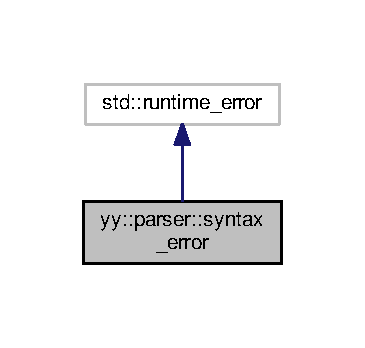
\includegraphics[width=175pt]{structyy_1_1parser_1_1syntax__error__inherit__graph}
\end{center}
\end{figure}


Collaboration diagram for yy\+:\+:parser\+:\+:syntax\+\_\+error\+:\nopagebreak
\begin{figure}[H]
\begin{center}
\leavevmode
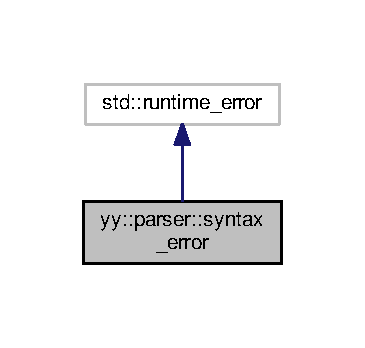
\includegraphics[width=175pt]{structyy_1_1parser_1_1syntax__error__coll__graph}
\end{center}
\end{figure}
\subsection*{Public Member Functions}
\begin{DoxyCompactItemize}
\item 
\hypertarget{structyy_1_1parser_1_1syntax__error_a41dabc53a4cf5a413dd1d93d415abc42}{}{\bfseries syntax\+\_\+error} (const std\+::string \&m)\label{structyy_1_1parser_1_1syntax__error_a41dabc53a4cf5a413dd1d93d415abc42}

\end{DoxyCompactItemize}


\subsection{Detailed Description}
Syntax errors thrown from user actions. 

The documentation for this struct was generated from the following file\+:\begin{DoxyCompactItemize}
\item 
inc/\hyperlink{parser_8h}{parser.\+h}\end{DoxyCompactItemize}

\hypertarget{classTest}{}\section{Test Class Reference}
\label{classTest}\index{Test@{Test}}


Class for test operations.  




{\ttfamily \#include $<$Test.\+h$>$}



Inheritance diagram for Test\+:\nopagebreak
\begin{figure}[H]
\begin{center}
\leavevmode
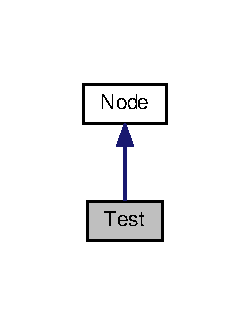
\includegraphics[width=120pt]{classTest__inherit__graph}
\end{center}
\end{figure}


Collaboration diagram for Test\+:\nopagebreak
\begin{figure}[H]
\begin{center}
\leavevmode
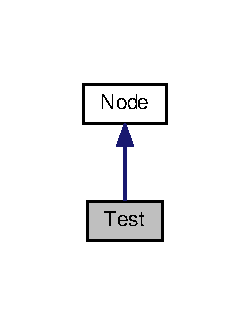
\includegraphics[width=120pt]{classTest__coll__graph}
\end{center}
\end{figure}
\subsection*{Public Types}
\begin{DoxyCompactItemize}
\item 
\hypertarget{classTest_a9e5d00cf02fb05573a6f97d14ebc154a}{}enum \hyperlink{classTest_a9e5d00cf02fb05573a6f97d14ebc154a}{Type} \{ \\*
{\bfseries Undefined}, 
{\bfseries Less\+Than}, 
{\bfseries Less\+Or\+Equal}, 
{\bfseries Greater\+Than}, 
\\*
{\bfseries Greater\+Or\+Equal}, 
{\bfseries Equal\+Equal}, 
{\bfseries Not\+Equal}, 
{\bfseries And}, 
\\*
{\bfseries Or}, 
{\bfseries Not}, 
{\bfseries False}, 
{\bfseries True}
 \}\label{classTest_a9e5d00cf02fb05573a6f97d14ebc154a}

\begin{DoxyCompactList}\small\item\em Defines types of Tests. \end{DoxyCompactList}\end{DoxyCompactItemize}
\subsection*{Public Member Functions}
\begin{DoxyCompactItemize}
\item 
\hypertarget{classTest_a99f2bbfac6c95612322b0f10e607ebe5}{}\hyperlink{classTest_a99f2bbfac6c95612322b0f10e607ebe5}{Test} ()\label{classTest_a99f2bbfac6c95612322b0f10e607ebe5}

\begin{DoxyCompactList}\small\item\em Default constructor. \end{DoxyCompactList}\item 
\hyperlink{classTest_aefafe8c714d1bbd89f09daf43793b465}{Test} (\hyperlink{classTest_a9e5d00cf02fb05573a6f97d14ebc154a}{Type} \hyperlink{classTest_add1faa7d527f515b973350d566772265}{type})
\begin{DoxyCompactList}\small\item\em Constructor with type. \end{DoxyCompactList}\item 
int \hyperlink{classTest_a579d613526a8fc37c15b461e2f07e65e}{execute} (\hyperlink{classEnvironment}{Environment} \&env)
\begin{DoxyCompactList}\small\item\em Executes the \hyperlink{classTest}{Test}. \end{DoxyCompactList}\item 
std\+::string \hyperlink{classTest_adeefe4160992fad5d3a52584f69a420d}{get\+Type} ()
\begin{DoxyCompactList}\small\item\em Converts type of node to string. \end{DoxyCompactList}\end{DoxyCompactItemize}
\subsection*{Protected Attributes}
\begin{DoxyCompactItemize}
\item 
\hypertarget{classTest_add1faa7d527f515b973350d566772265}{}\hyperlink{classTest_a9e5d00cf02fb05573a6f97d14ebc154a}{Type} \hyperlink{classTest_add1faa7d527f515b973350d566772265}{type}\label{classTest_add1faa7d527f515b973350d566772265}

\begin{DoxyCompactList}\small\item\em \hyperlink{classTest}{Test} type. \end{DoxyCompactList}\end{DoxyCompactItemize}


\subsection{Detailed Description}
Class for test operations. 

\begin{DoxyAuthor}{Author}
Jim Ahlstrand 
\end{DoxyAuthor}
\begin{DoxyRefDesc}{Todo}
\item[\hyperlink{todo__todo000003}{Todo}]add test for number of children, test can have max 2 \end{DoxyRefDesc}


\subsection{Constructor \& Destructor Documentation}
\hypertarget{classTest_aefafe8c714d1bbd89f09daf43793b465}{}\index{Test@{Test}!Test@{Test}}
\index{Test@{Test}!Test@{Test}}
\subsubsection[{Test}]{\setlength{\rightskip}{0pt plus 5cm}Test\+::\+Test (
\begin{DoxyParamCaption}
\item[{{\bf Type}}]{type}
\end{DoxyParamCaption}
)}\label{classTest_aefafe8c714d1bbd89f09daf43793b465}


Constructor with type. 


\begin{DoxyParams}{Parameters}
{\em type} & \hyperlink{classTest}{Test} type of enum Type \\
\hline
\end{DoxyParams}


\subsection{Member Function Documentation}
\hypertarget{classTest_a579d613526a8fc37c15b461e2f07e65e}{}\index{Test@{Test}!execute@{execute}}
\index{execute@{execute}!Test@{Test}}
\subsubsection[{execute}]{\setlength{\rightskip}{0pt plus 5cm}int Test\+::execute (
\begin{DoxyParamCaption}
\item[{{\bf Environment} \&}]{env}
\end{DoxyParamCaption}
)\hspace{0.3cm}{\ttfamily [virtual]}}\label{classTest_a579d613526a8fc37c15b461e2f07e65e}


Executes the \hyperlink{classTest}{Test}. 


\begin{DoxyParams}{Parameters}
{\em env} & current \hyperlink{classEnvironment}{Environment} \\
\hline
\end{DoxyParams}
\begin{DoxyReturn}{Returns}
integer value of the node 
\end{DoxyReturn}


Reimplemented from \hyperlink{classNode_acc70d98952c4b061bc433c00180b7011}{Node}.

\hypertarget{classTest_adeefe4160992fad5d3a52584f69a420d}{}\index{Test@{Test}!get\+Type@{get\+Type}}
\index{get\+Type@{get\+Type}!Test@{Test}}
\subsubsection[{get\+Type}]{\setlength{\rightskip}{0pt plus 5cm}std\+::string Test\+::get\+Type (
\begin{DoxyParamCaption}
{}
\end{DoxyParamCaption}
)\hspace{0.3cm}{\ttfamily [virtual]}}\label{classTest_adeefe4160992fad5d3a52584f69a420d}


Converts type of node to string. 

\begin{DoxyReturn}{Returns}
string type of the node 
\end{DoxyReturn}


Reimplemented from \hyperlink{classNode_abce0a9ddac6a5e2c0e546dbe6af02e3d}{Node}.



The documentation for this class was generated from the following files\+:\begin{DoxyCompactItemize}
\item 
inc/Test.\+h\item 
src/Test.\+cpp\end{DoxyCompactItemize}

\hypertarget{structyy_1_1parser_1_1token}{}\section{yy\+:\+:parser\+:\+:token Struct Reference}
\label{structyy_1_1parser_1_1token}\index{yy\+::parser\+::token@{yy\+::parser\+::token}}


Tokens.  




{\ttfamily \#include $<$parser.\+h$>$}

\subsection*{Public Types}
\begin{DoxyCompactItemize}
\item 
\hypertarget{structyy_1_1parser_1_1token_a90b63e7f9dd7177dd3bf01c58c408475}{}enum {\bfseries yytokentype} \{ \\*
{\bfseries E\+N\+D} = 0, 
{\bfseries S\+T\+R} = 258, 
{\bfseries N\+U\+M} = 259, 
{\bfseries N\+A\+M\+E} = 260, 
\\*
{\bfseries W\+H\+I\+L\+E} = 261, 
{\bfseries F\+O\+R} = 262, 
{\bfseries D\+O} = 263, 
{\bfseries I\+F} = 264, 
\\*
{\bfseries E\+L\+S\+E} = 265, 
{\bfseries E\+L\+S\+E\+I\+F} = 266, 
{\bfseries T\+H\+E\+N} = 267, 
{\bfseries R\+E\+T\+U\+R\+N} = 268, 
\\*
{\bfseries B\+R\+E\+A\+K} = 269, 
{\bfseries \+\_\+\+F\+A\+L\+S\+E} = 270, 
{\bfseries \+\_\+\+T\+R\+U\+E} = 271, 
{\bfseries \+\_\+\+E\+N\+D} = 272, 
\\*
{\bfseries I\+N} = 273, 
{\bfseries L\+O\+C\+A\+L} = 274, 
{\bfseries N\+I\+L} = 275, 
{\bfseries R\+E\+P} = 276, 
\\*
{\bfseries U\+N\+T\+I\+L} = 277, 
{\bfseries S\+E\+M\+C\+O\+L} = 278, 
{\bfseries E\+Q} = 279, 
{\bfseries C\+O\+M} = 280, 
\\*
{\bfseries D\+O\+T} = 281, 
{\bfseries C\+O\+L} = 282, 
{\bfseries B\+R\+K\+O\+P\+N} = 283, 
{\bfseries B\+R\+K\+C\+L\+S} = 284, 
\\*
{\bfseries T\+R\+I\+D\+O\+T} = 285, 
{\bfseries P\+A\+R\+O\+P\+N} = 286, 
{\bfseries P\+A\+R\+C\+L\+S} = 287, 
{\bfseries C\+U\+R\+O\+P\+N} = 288, 
\\*
{\bfseries C\+U\+R\+C\+L\+S} = 289, 
{\bfseries F\+U\+N\+C} = 290, 
{\bfseries O\+R} = 291, 
{\bfseries A\+N\+D} = 292, 
\\*
{\bfseries L\+E\+S\+S} = 293, 
{\bfseries G\+R\+E\+A\+T} = 294, 
{\bfseries L\+E\+S\+S\+E\+Q} = 295, 
{\bfseries G\+R\+E\+A\+T\+E\+Q} = 296, 
\\*
{\bfseries E\+Q\+E\+Q} = 297, 
{\bfseries N\+O\+T\+E\+Q} = 298, 
{\bfseries D\+D\+O\+T} = 299, 
{\bfseries P\+L\+U\+S} = 300, 
\\*
{\bfseries M\+I\+N\+U\+S} = 301, 
{\bfseries M\+U\+L\+T} = 302, 
{\bfseries D\+I\+V} = 303, 
{\bfseries M\+O\+D} = 304, 
\\*
{\bfseries N\+O\+T} = 305, 
{\bfseries H\+A\+S\+H} = 306, 
{\bfseries P\+O\+W} = 307
 \}\label{structyy_1_1parser_1_1token_a90b63e7f9dd7177dd3bf01c58c408475}

\end{DoxyCompactItemize}


\subsection{Detailed Description}
Tokens. 

The documentation for this struct was generated from the following file\+:\begin{DoxyCompactItemize}
\item 
inc/\hyperlink{parser_8h}{parser.\+h}\end{DoxyCompactItemize}

\hypertarget{unionyy_1_1parser_1_1union__type}{}\section{yy\+:\+:parser\+:\+:union\+\_\+type Union Reference}
\label{unionyy_1_1parser_1_1union__type}\index{yy\+::parser\+::union\+\_\+type@{yy\+::parser\+::union\+\_\+type}}


An auxiliary type to compute the largest semantic type.  




{\ttfamily \#include $<$parser.\+h$>$}

\subsection*{Public Attributes}
\begin{DoxyCompactItemize}
\item 
\hypertarget{unionyy_1_1parser_1_1union__type_a0db9b7b9325335136722f9966c455746}{}char {\bfseries dummy1} \mbox{[}sizeof(\hyperlink{classNode}{Node} $\ast$)\mbox{]}\label{unionyy_1_1parser_1_1union__type_a0db9b7b9325335136722f9966c455746}

\item 
\hypertarget{unionyy_1_1parser_1_1union__type_a77671989075b3b4f942b9d82ccc645c8}{}char {\bfseries dummy2} \mbox{[}sizeof(string)\mbox{]}\label{unionyy_1_1parser_1_1union__type_a77671989075b3b4f942b9d82ccc645c8}

\end{DoxyCompactItemize}


\subsection{Detailed Description}
An auxiliary type to compute the largest semantic type. 

The documentation for this union was generated from the following file\+:\begin{DoxyCompactItemize}
\item 
inc/\hyperlink{parser_8h}{parser.\+h}\end{DoxyCompactItemize}

\hypertarget{structyy_1_1variant}{}\section{yy\+:\+:variant$<$ S $>$ Struct Template Reference}
\label{structyy_1_1variant}\index{yy\+::variant$<$ S $>$@{yy\+::variant$<$ S $>$}}


{\ttfamily \#include $<$parser.\+h$>$}

\subsection*{Public Types}
\begin{DoxyCompactItemize}
\item 
\hypertarget{structyy_1_1variant_afbd75aee339bd9fa06e6fa8f320cecd3}{}typedef \hyperlink{structyy_1_1variant}{variant}$<$ S $>$ \hyperlink{structyy_1_1variant_afbd75aee339bd9fa06e6fa8f320cecd3}{self\+\_\+type}\label{structyy_1_1variant_afbd75aee339bd9fa06e6fa8f320cecd3}

\begin{DoxyCompactList}\small\item\em Type of $\ast$this. \end{DoxyCompactList}\end{DoxyCompactItemize}
\subsection*{Public Member Functions}
\begin{DoxyCompactItemize}
\item 
\hypertarget{structyy_1_1variant_ad89e5bb6a0418c8065b9d0d2b05b2d23}{}\hyperlink{structyy_1_1variant_ad89e5bb6a0418c8065b9d0d2b05b2d23}{variant} ()\label{structyy_1_1variant_ad89e5bb6a0418c8065b9d0d2b05b2d23}

\begin{DoxyCompactList}\small\item\em Empty construction. \end{DoxyCompactList}\item 
\hypertarget{structyy_1_1variant_a8022c28bb598dd69dbb3f14db4c9cc1f}{}{\footnotesize template$<$typename T $>$ }\\\hyperlink{structyy_1_1variant_a8022c28bb598dd69dbb3f14db4c9cc1f}{variant} (const T \&t)\label{structyy_1_1variant_a8022c28bb598dd69dbb3f14db4c9cc1f}

\begin{DoxyCompactList}\small\item\em Construct and fill. \end{DoxyCompactList}\item 
\hypertarget{structyy_1_1variant_a41eed194f0196ede63cd451e9b7835e3}{}\hyperlink{structyy_1_1variant_a41eed194f0196ede63cd451e9b7835e3}{$\sim$variant} ()\label{structyy_1_1variant_a41eed194f0196ede63cd451e9b7835e3}

\begin{DoxyCompactList}\small\item\em Destruction, allowed only if empty. \end{DoxyCompactList}\item 
\hypertarget{structyy_1_1variant_a182022d05c0d80a410ba83996ec0b637}{}{\footnotesize template$<$typename T $>$ }\\T \& \hyperlink{structyy_1_1variant_a182022d05c0d80a410ba83996ec0b637}{build} ()\label{structyy_1_1variant_a182022d05c0d80a410ba83996ec0b637}

\begin{DoxyCompactList}\small\item\em Instantiate an empty {\itshape T} in here. \end{DoxyCompactList}\item 
\hypertarget{structyy_1_1variant_ae638b88f2eb38e93f0cb4b74bda844fe}{}{\footnotesize template$<$typename T $>$ }\\T \& \hyperlink{structyy_1_1variant_ae638b88f2eb38e93f0cb4b74bda844fe}{build} (const T \&t)\label{structyy_1_1variant_ae638b88f2eb38e93f0cb4b74bda844fe}

\begin{DoxyCompactList}\small\item\em Instantiate a {\itshape T} in here from {\itshape t}. \end{DoxyCompactList}\item 
\hypertarget{structyy_1_1variant_a7fae4866c8d57a6f2ea30e9926e367cd}{}{\footnotesize template$<$typename T $>$ }\\T \& \hyperlink{structyy_1_1variant_a7fae4866c8d57a6f2ea30e9926e367cd}{as} ()\label{structyy_1_1variant_a7fae4866c8d57a6f2ea30e9926e367cd}

\begin{DoxyCompactList}\small\item\em Accessor to a built {\itshape T}. \end{DoxyCompactList}\item 
\hypertarget{structyy_1_1variant_a7930977f8a1b707c687daec8b0d76e70}{}{\footnotesize template$<$typename T $>$ }\\const T \& \hyperlink{structyy_1_1variant_a7930977f8a1b707c687daec8b0d76e70}{as} () const \label{structyy_1_1variant_a7930977f8a1b707c687daec8b0d76e70}

\begin{DoxyCompactList}\small\item\em Const accessor to a built {\itshape T} (for printer). \end{DoxyCompactList}\item 
{\footnotesize template$<$typename T $>$ }\\void \hyperlink{structyy_1_1variant_ac43b5ffdcedbda5462c53832027707ac}{swap} (\hyperlink{structyy_1_1variant_afbd75aee339bd9fa06e6fa8f320cecd3}{self\+\_\+type} \&other)
\item 
{\footnotesize template$<$typename T $>$ }\\void \hyperlink{structyy_1_1variant_ae71b4ef21f1446b328b9d93dbc6806e1}{move} (\hyperlink{structyy_1_1variant_afbd75aee339bd9fa06e6fa8f320cecd3}{self\+\_\+type} \&other)
\item 
\hypertarget{structyy_1_1variant_a526d966e2923f6ae1d3fab2e1eac5311}{}{\footnotesize template$<$typename T $>$ }\\void \hyperlink{structyy_1_1variant_a526d966e2923f6ae1d3fab2e1eac5311}{copy} (const \hyperlink{structyy_1_1variant_afbd75aee339bd9fa06e6fa8f320cecd3}{self\+\_\+type} \&other)\label{structyy_1_1variant_a526d966e2923f6ae1d3fab2e1eac5311}

\begin{DoxyCompactList}\small\item\em Copy the content of {\itshape other} to this. \end{DoxyCompactList}\item 
\hypertarget{structyy_1_1variant_a20a07d58bf12eda819ad013c5d9853cb}{}{\footnotesize template$<$typename T $>$ }\\void \hyperlink{structyy_1_1variant_a20a07d58bf12eda819ad013c5d9853cb}{destroy} ()\label{structyy_1_1variant_a20a07d58bf12eda819ad013c5d9853cb}

\begin{DoxyCompactList}\small\item\em Destroy the stored {\itshape T}. \end{DoxyCompactList}\end{DoxyCompactItemize}


\subsection{Detailed Description}
\subsubsection*{template$<$size\+\_\+t S$>$struct yy\+::variant$<$ S $>$}

A char\mbox{[}S\mbox{]} buffer to store and retrieve objects.

Sort of a variant, but does not keep track of the nature of the stored data, since that knowledge is available via the current state. 

\subsection{Member Function Documentation}
\hypertarget{structyy_1_1variant_ae71b4ef21f1446b328b9d93dbc6806e1}{}\index{yy\+::variant@{yy\+::variant}!move@{move}}
\index{move@{move}!yy\+::variant@{yy\+::variant}}
\subsubsection[{move}]{\setlength{\rightskip}{0pt plus 5cm}template$<$size\+\_\+t S$>$ template$<$typename T $>$ void {\bf yy\+::variant}$<$ S $>$\+::move (
\begin{DoxyParamCaption}
\item[{{\bf self\+\_\+type} \&}]{other}
\end{DoxyParamCaption}
)\hspace{0.3cm}{\ttfamily [inline]}}\label{structyy_1_1variant_ae71b4ef21f1446b328b9d93dbc6806e1}
Move the content of {\itshape other} to this.

Destroys {\itshape other}. \hypertarget{structyy_1_1variant_ac43b5ffdcedbda5462c53832027707ac}{}\index{yy\+::variant@{yy\+::variant}!swap@{swap}}
\index{swap@{swap}!yy\+::variant@{yy\+::variant}}
\subsubsection[{swap}]{\setlength{\rightskip}{0pt plus 5cm}template$<$size\+\_\+t S$>$ template$<$typename T $>$ void {\bf yy\+::variant}$<$ S $>$\+::swap (
\begin{DoxyParamCaption}
\item[{{\bf self\+\_\+type} \&}]{other}
\end{DoxyParamCaption}
)\hspace{0.3cm}{\ttfamily [inline]}}\label{structyy_1_1variant_ac43b5ffdcedbda5462c53832027707ac}
Swap the content with {\itshape other}, of same type.

Both variants must be built beforehand, because swapping the actual data requires reading it (with \hyperlink{structyy_1_1variant_a7fae4866c8d57a6f2ea30e9926e367cd}{as()}), and this is not possible on unconstructed variants\+: it would require some dynamic testing, which should not be the variant\textquotesingle{}s responsability. Swapping between built and (possibly) non-\/built is done with \hyperlink{structyy_1_1variant_ae71b4ef21f1446b328b9d93dbc6806e1}{variant\+::move} (). 

The documentation for this struct was generated from the following file\+:\begin{DoxyCompactItemize}
\item 
inc/\hyperlink{parser_8h}{parser.\+h}\end{DoxyCompactItemize}

\hypertarget{structyy__buffer__state}{}\section{yy\+\_\+buffer\+\_\+state Struct Reference}
\label{structyy__buffer__state}\index{yy\+\_\+buffer\+\_\+state@{yy\+\_\+buffer\+\_\+state}}
\subsection*{Public Attributes}
\begin{DoxyCompactItemize}
\item 
\hypertarget{structyy__buffer__state_a4360acfb226a1fc240ab2be17dd6beda}{}F\+I\+L\+E $\ast$ {\bfseries yy\+\_\+input\+\_\+file}\label{structyy__buffer__state_a4360acfb226a1fc240ab2be17dd6beda}

\item 
\hypertarget{structyy__buffer__state_a0d25458e69eb22207fc633a1255d099d}{}char $\ast$ {\bfseries yy\+\_\+ch\+\_\+buf}\label{structyy__buffer__state_a0d25458e69eb22207fc633a1255d099d}

\item 
\hypertarget{structyy__buffer__state_a8435c3f786bbb55d21d0174e4cfc22a0}{}char $\ast$ {\bfseries yy\+\_\+buf\+\_\+pos}\label{structyy__buffer__state_a8435c3f786bbb55d21d0174e4cfc22a0}

\item 
\hypertarget{structyy__buffer__state_a48302f5f3477a9c78bbddf56d356ef54}{}yy\+\_\+size\+\_\+t {\bfseries yy\+\_\+buf\+\_\+size}\label{structyy__buffer__state_a48302f5f3477a9c78bbddf56d356ef54}

\item 
\hypertarget{structyy__buffer__state_afcc44872643f513e79b43c2b1f334a67}{}yy\+\_\+size\+\_\+t {\bfseries yy\+\_\+n\+\_\+chars}\label{structyy__buffer__state_afcc44872643f513e79b43c2b1f334a67}

\item 
\hypertarget{structyy__buffer__state_a80ce2431c70dc4f89ced487f18449465}{}int {\bfseries yy\+\_\+is\+\_\+our\+\_\+buffer}\label{structyy__buffer__state_a80ce2431c70dc4f89ced487f18449465}

\item 
\hypertarget{structyy__buffer__state_abf5c70eea75581b58c0ee7bd31b14490}{}int {\bfseries yy\+\_\+is\+\_\+interactive}\label{structyy__buffer__state_abf5c70eea75581b58c0ee7bd31b14490}

\item 
\hypertarget{structyy__buffer__state_a9d60c60af6e1a6f69de16871fd64f85f}{}int {\bfseries yy\+\_\+at\+\_\+bol}\label{structyy__buffer__state_a9d60c60af6e1a6f69de16871fd64f85f}

\item 
int \hyperlink{structyy__buffer__state_a818e94bc9c766e683c60df1e9fd01199}{yy\+\_\+bs\+\_\+lineno}
\begin{DoxyCompactList}\small\item\em The line count. \end{DoxyCompactList}\item 
int \hyperlink{structyy__buffer__state_a10c4fcd8be759e6bf11e6d3e8cdb0307}{yy\+\_\+bs\+\_\+column}
\begin{DoxyCompactList}\small\item\em The column count. \end{DoxyCompactList}\item 
\hypertarget{structyy__buffer__state_a63d2afbb1d79a3fc63df9e12626f827d}{}int {\bfseries yy\+\_\+fill\+\_\+buffer}\label{structyy__buffer__state_a63d2afbb1d79a3fc63df9e12626f827d}

\item 
\hypertarget{structyy__buffer__state_a70fd925d37a2f0454fbd0def675d106c}{}int {\bfseries yy\+\_\+buffer\+\_\+status}\label{structyy__buffer__state_a70fd925d37a2f0454fbd0def675d106c}

\end{DoxyCompactItemize}


\subsection{Member Data Documentation}
\hypertarget{structyy__buffer__state_a10c4fcd8be759e6bf11e6d3e8cdb0307}{}\index{yy\+\_\+buffer\+\_\+state@{yy\+\_\+buffer\+\_\+state}!yy\+\_\+bs\+\_\+column@{yy\+\_\+bs\+\_\+column}}
\index{yy\+\_\+bs\+\_\+column@{yy\+\_\+bs\+\_\+column}!yy\+\_\+buffer\+\_\+state@{yy\+\_\+buffer\+\_\+state}}
\subsubsection[{yy\+\_\+bs\+\_\+column}]{\setlength{\rightskip}{0pt plus 5cm}int yy\+\_\+buffer\+\_\+state\+::yy\+\_\+bs\+\_\+column}\label{structyy__buffer__state_a10c4fcd8be759e6bf11e6d3e8cdb0307}


The column count. 

\hypertarget{structyy__buffer__state_a818e94bc9c766e683c60df1e9fd01199}{}\index{yy\+\_\+buffer\+\_\+state@{yy\+\_\+buffer\+\_\+state}!yy\+\_\+bs\+\_\+lineno@{yy\+\_\+bs\+\_\+lineno}}
\index{yy\+\_\+bs\+\_\+lineno@{yy\+\_\+bs\+\_\+lineno}!yy\+\_\+buffer\+\_\+state@{yy\+\_\+buffer\+\_\+state}}
\subsubsection[{yy\+\_\+bs\+\_\+lineno}]{\setlength{\rightskip}{0pt plus 5cm}int yy\+\_\+buffer\+\_\+state\+::yy\+\_\+bs\+\_\+lineno}\label{structyy__buffer__state_a818e94bc9c766e683c60df1e9fd01199}


The line count. 



The documentation for this struct was generated from the following files\+:\begin{DoxyCompactItemize}
\item 
inc/scanner.\+h\item 
src/scanner.\+cpp\end{DoxyCompactItemize}

\hypertarget{structyy__trans__info}{}\section{yy\+\_\+trans\+\_\+info Struct Reference}
\label{structyy__trans__info}\index{yy\+\_\+trans\+\_\+info@{yy\+\_\+trans\+\_\+info}}
\subsection*{Public Attributes}
\begin{DoxyCompactItemize}
\item 
\hypertarget{structyy__trans__info_a5c9f61e770deef50bd4e697310342fe9}{}flex\+\_\+int32\+\_\+t {\bfseries yy\+\_\+verify}\label{structyy__trans__info_a5c9f61e770deef50bd4e697310342fe9}

\item 
\hypertarget{structyy__trans__info_ae0715250c2bef261e596e77e0030f13e}{}flex\+\_\+int32\+\_\+t {\bfseries yy\+\_\+nxt}\label{structyy__trans__info_ae0715250c2bef261e596e77e0030f13e}

\end{DoxyCompactItemize}


The documentation for this struct was generated from the following file\+:\begin{DoxyCompactItemize}
\item 
src/scanner.\+cpp\end{DoxyCompactItemize}

\chapter{File Documentation}
\hypertarget{parser_8h}{}\section{inc/parser.h File Reference}
\label{parser_8h}\index{inc/parser.\+h@{inc/parser.\+h}}
{\ttfamily \#include \char`\"{}Node.\+h\char`\"{}}\\*
{\ttfamily \#include \char`\"{}Test.\+h\char`\"{}}\\*
{\ttfamily \#include \char`\"{}Loop.\+h\char`\"{}}\\*
{\ttfamily \#include \char`\"{}Binop.\+h\char`\"{}}\\*
{\ttfamily \#include \char`\"{}Condition.\+h\char`\"{}}\\*
{\ttfamily \#include \char`\"{}Environment.\+h\char`\"{}}\\*
{\ttfamily \#include $<$vector$>$}\\*
{\ttfamily \#include $<$iostream$>$}\\*
{\ttfamily \#include $<$stdexcept$>$}\\*
{\ttfamily \#include $<$string$>$}\\*
{\ttfamily \#include \char`\"{}stack.\+hh\char`\"{}}\\*
{\ttfamily \#include $<$cassert$>$}\\*
Include dependency graph for parser.\+h\+:\nopagebreak
\begin{figure}[H]
\begin{center}
\leavevmode
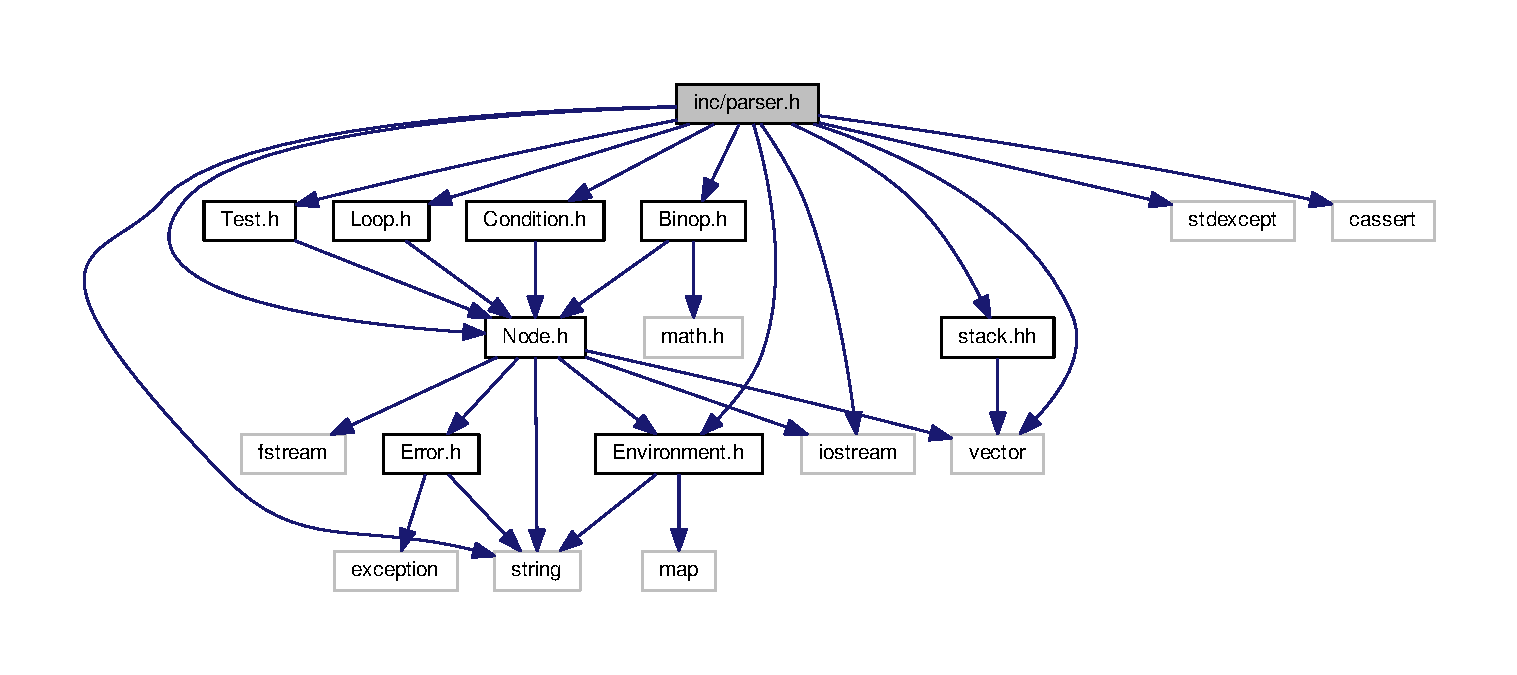
\includegraphics[width=350pt]{parser_8h__incl}
\end{center}
\end{figure}
This graph shows which files directly or indirectly include this file\+:\nopagebreak
\begin{figure}[H]
\begin{center}
\leavevmode
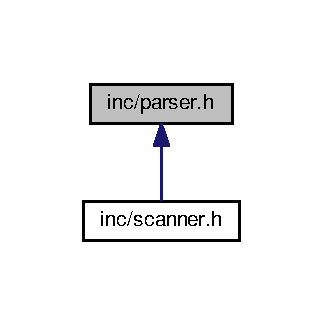
\includegraphics[width=155pt]{parser_8h__dep__incl}
\end{center}
\end{figure}
\subsection*{Classes}
\begin{DoxyCompactItemize}
\item 
struct \hyperlink{structyy_1_1variant}{yy\+::variant$<$ S $>$}
\item 
class \hyperlink{classyy_1_1parser}{yy\+::parser}
\begin{DoxyCompactList}\small\item\em A Bison parser. \end{DoxyCompactList}\item 
union \hyperlink{unionyy_1_1parser_1_1union__type}{yy\+::parser\+::union\+\_\+type}
\begin{DoxyCompactList}\small\item\em An auxiliary type to compute the largest semantic type. \end{DoxyCompactList}\item 
struct \hyperlink{structyy_1_1parser_1_1syntax__error}{yy\+::parser\+::syntax\+\_\+error}
\begin{DoxyCompactList}\small\item\em Syntax errors thrown from user actions. \end{DoxyCompactList}\item 
struct \hyperlink{structyy_1_1parser_1_1token}{yy\+::parser\+::token}
\begin{DoxyCompactList}\small\item\em Tokens. \end{DoxyCompactList}\item 
struct \hyperlink{structyy_1_1parser_1_1basic__symbol}{yy\+::parser\+::basic\+\_\+symbol$<$ Base $>$}
\item 
struct \hyperlink{structyy_1_1parser_1_1by__type}{yy\+::parser\+::by\+\_\+type}
\begin{DoxyCompactList}\small\item\em Type access provider for token (enum) based symbols. \end{DoxyCompactList}\end{DoxyCompactItemize}
\subsection*{Macros}
\begin{DoxyCompactItemize}
\item 
\hypertarget{parser_8h_afd603ddcf170a7d46a33d9d780d18a4b}{}\#define {\bfseries Y\+Y\+A\+S\+S\+E\+R\+T}~assert\label{parser_8h_afd603ddcf170a7d46a33d9d780d18a4b}

\item 
\hypertarget{parser_8h_a9b07478214400ec2e160dffd1d945266}{}\#define {\bfseries Y\+Y\+\_\+\+A\+T\+T\+R\+I\+B\+U\+T\+E}(Spec)~/$\ast$ empty $\ast$/\label{parser_8h_a9b07478214400ec2e160dffd1d945266}

\item 
\hypertarget{parser_8h_ad1405f082b8df6353a9d53c9709c4d03}{}\#define {\bfseries Y\+Y\+\_\+\+A\+T\+T\+R\+I\+B\+U\+T\+E\+\_\+\+P\+U\+R\+E}~Y\+Y\+\_\+\+A\+T\+T\+R\+I\+B\+U\+T\+E ((\+\_\+\+\_\+pure\+\_\+\+\_\+))\label{parser_8h_ad1405f082b8df6353a9d53c9709c4d03}

\item 
\hypertarget{parser_8h_ab312a884bd41ff11bbd1aa6c1a0e1b0a}{}\#define {\bfseries Y\+Y\+\_\+\+A\+T\+T\+R\+I\+B\+U\+T\+E\+\_\+\+U\+N\+U\+S\+E\+D}~Y\+Y\+\_\+\+A\+T\+T\+R\+I\+B\+U\+T\+E ((\+\_\+\+\_\+unused\+\_\+\+\_\+))\label{parser_8h_ab312a884bd41ff11bbd1aa6c1a0e1b0a}

\item 
\hypertarget{parser_8h_afdc60192553b70b37149691b71022d5a}{}\#define {\bfseries \+\_\+\+Noreturn}~Y\+Y\+\_\+\+A\+T\+T\+R\+I\+B\+U\+T\+E ((\+\_\+\+\_\+noreturn\+\_\+\+\_\+))\label{parser_8h_afdc60192553b70b37149691b71022d5a}

\item 
\hypertarget{parser_8h_a33c61e326f5675cc74eb9e1a6906595c}{}\#define {\bfseries Y\+Y\+U\+S\+E}(E)~((void) (E))\label{parser_8h_a33c61e326f5675cc74eb9e1a6906595c}

\item 
\hypertarget{parser_8h_a6d890db48971847b837a6a1397c9059a}{}\#define {\bfseries Y\+Y\+\_\+\+I\+N\+I\+T\+I\+A\+L\+\_\+\+V\+A\+L\+U\+E}(Value)~Value\label{parser_8h_a6d890db48971847b837a6a1397c9059a}

\item 
\hypertarget{parser_8h_a145ddbb780f86b5f35ddfffb23e62d4d}{}\#define {\bfseries Y\+Y\+\_\+\+I\+G\+N\+O\+R\+E\+\_\+\+M\+A\+Y\+B\+E\+\_\+\+U\+N\+I\+N\+I\+T\+I\+A\+L\+I\+Z\+E\+D\+\_\+\+B\+E\+G\+I\+N}\label{parser_8h_a145ddbb780f86b5f35ddfffb23e62d4d}

\item 
\hypertarget{parser_8h_a2b2abbe8d335b7933a69ac2f05a015d2}{}\#define {\bfseries Y\+Y\+\_\+\+I\+G\+N\+O\+R\+E\+\_\+\+M\+A\+Y\+B\+E\+\_\+\+U\+N\+I\+N\+I\+T\+I\+A\+L\+I\+Z\+E\+D\+\_\+\+E\+N\+D}\label{parser_8h_a2b2abbe8d335b7933a69ac2f05a015d2}

\item 
\hypertarget{parser_8h_a853b3bfad6d2b2ff693dce81182e0c2e}{}\#define {\bfseries Y\+Y\+D\+E\+B\+U\+G}~0\label{parser_8h_a853b3bfad6d2b2ff693dce81182e0c2e}

\end{DoxyCompactItemize}


\subsection{Detailed Description}
Define the \hyperlink{classyy_1_1parser}{yy\+::parser} class. 
\hypertarget{src_2stack_8hh}{}\section{src/stack.hh File Reference}
\label{src_2stack_8hh}\index{src/stack.\+hh@{src/stack.\+hh}}


Define the \hyperlink{classyy_1_1stack}{yy\+::stack} class.  


{\ttfamily \#include $<$vector$>$}\\*
Include dependency graph for stack.\+hh\+:\nopagebreak
\begin{figure}[H]
\begin{center}
\leavevmode
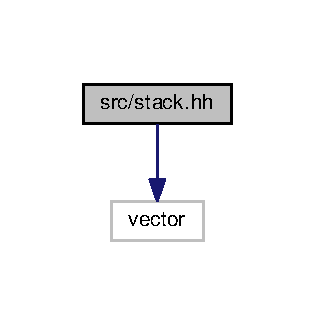
\includegraphics[width=151pt]{src_2stack_8hh__incl}
\end{center}
\end{figure}
\subsection*{Classes}
\begin{DoxyCompactItemize}
\item 
class \hyperlink{classyy_1_1stack}{yy\+::stack$<$ T, S $>$}
\item 
class \hyperlink{classyy_1_1slice}{yy\+::slice$<$ T, S $>$}
\begin{DoxyCompactList}\small\item\em Present a slice of the top of a stack. \end{DoxyCompactList}\end{DoxyCompactItemize}


\subsection{Detailed Description}
Define the \hyperlink{classyy_1_1stack}{yy\+::stack} class. 


%--- End generated contents ---

% Index
\backmatter
\newpage
\phantomsection
\clearemptydoublepage
\addcontentsline{toc}{chapter}{Index}
\printindex

\end{document}
